
\chapter{HASIL DAN PEMBAHASAN}

\section{Ekplorasi Dataset}

    Penelitian ini menggunakan data video dalam format video (.avi). Jumlah data berjumlah 319 video yang terdiri dari 
    pengemudi pria berjmlah 163 video dan wanita berjumlah 156 video dengan resolusi 640 x 480 piksel dan kecepatan tiga 
    puluh \textit{frame per second} (FPS). Dataset ini memiliki beberapa penjelesan terkait dengan kondisi video, yaitu:
    
    \begin{enumerate}
        \item \textit{Participant Number}: Variabel yang memberikan informasi terkait dengan nomor partisipasi dalam dataset.
        \item \textit{Action}: Memberikan informasi terkait hal yang terjadi pada pengemudi.
        \item \textit{Scarf}:  Memberikan informasi apakah pengendara menggunakan syal atau tidak.
        \item \textit{Background Movement}: Memberitahukan kondisi latar belakang video, bergerak atau tidak.

         \item  \textit{Glasses}: Jenis kacamata yang digunakan.
        
        \item \textit{Lighting}: Memberikan informasi kondisi pencahayaan.
        
        \item  \textit{Ethnicity}: Jenis etnis pengendara.

        \item  \textit{Duration}: Durasi video pengendara dengan satuan detik
        
        
    \end{enumerate}

  


    Penjelesan dataset untuk setiap videonya disajikan dalam Tabel \ref{Penjelasan Dataset} berikut.

  \begin{table}[htbp]
        \centering
        \caption{Penjelasan Dataset}
        \label{Penjelasan Dataset}
    \scriptsize
        \begin{tabular}{p{0.5cm} p{1.2 cm} p{1.2 cm} p{1.1cm} p{1.3 cm} {0.5 cm} {1.0 cm} {0.5 cm}{0.7cm}{0.6cm} }
        \hline
        \textbf{No.} & \textbf{Participant Number} & \textbf{Action} & \textbf{Scarf} & \textbf{BG Movement} & \textbf{Glasses} & \textbf{Lighting} & \textbf{Ethnicity} & \textbf{Durasi} \\
        \hline

        \hline
        1 & 1 & Talking & No & No & No Glasses & Sunny & Caucasian & 24 s\\
        2 & 1 & Yawning & No & No & Sun glasses & Sunny & Caucasian & 14 s\\
        3 & 1 & Normal & No & Yes & Prescription & Sunny & Middle Eastern & 16 s\\
        4 & 1 & Yawning & No & No & Prescription & Sunny & Caucasian & 14 s\\
        5 & 2 & Yawning & No & Yes & No Glasses & Sunny & Caucasian & 15 s \\
        6 & 2 & Talking & No & No & No Glasses & Sunny & Caucasian & 18 s\\
        7 & 2 & Yawning & No & No & Sun glasses & Sunny & Caucasian  & 14 s\\
        8 & 3 & Normal & No & Yes & Prescription & Sunny & Middle Eastern & 15 s\\
        ... &... & ... & ... & ... & ... & ... & ...& ...  \\
        ... &... & ... & ... & ... & ... & ... & ... & ... \\
        ... &... & ... & ... & ... & ... & ... & ... & ...  \\
        156 &142 & Yawning & No & No & No Glasses & Sunny & Middle Eastern & 22 s\\
        157 & 145 & Yawning & No & No & No Glasses & Sunny & Middle Eastern & 20 s\\
        158 &148 & Yawning & No & Yes & No Glasses & Sunny & Caucasian  & 16 s\\
        159 &151 & Yawning & No & No & No Glasses & Sunny & Caucasian& 19 s \\
        160 &154 & Yawning & No & Yes & No Glasses & Sunny & Middle Eastern & 23 s\\
        161 &157 & Yawning & No & Yes & No Glasses & Sunny & Middle Eastern & 37 s\\
        162 &160 & Yawning & No & Yes & Prescription & Sunny & Middle Eastern & 18 s\\
        \hline
        \end{tabular}
        \end{table}

    Contoh dataset awal yang berupa video ditampilkan seperti Gambar \ref{Dataset Video} berikut.

     \begin{figure}[H]
         \centering
             \centering
             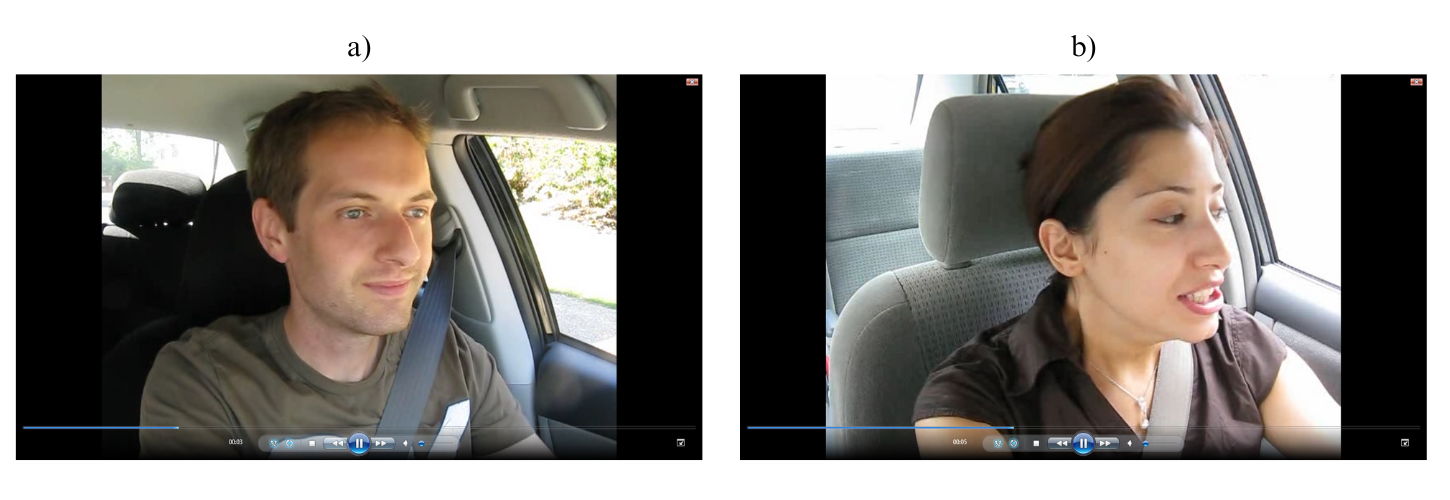
\includegraphics[width=\textwidth]{figures/bab4/data video.png}
             \caption{a) \textit{Male}, b) \textit{Female}}
             \label{Dataset Video}
     \end{figure}


    Data video diekstrak menjadi gambar dengan menggunakan nilai EAR dan MAR, setiap foto hasil ektraksi akan langsung otomatis masuk dalam folder sesuai dengan kelas yang telah ditentukan. Penentuan kelas sebuah gambar dikelompokkan pada kategori kelas tetentu di peroleh berdasarkan kondisi nilai EAR dan MAR seperti yang tertulis sebagai berikut.

    \begin{enumerate}
        \item    Jika nilai EAR pada \textit{frame} tersebut lebih kecil dari EAR \textit{threshold} dan MAR lebih besar MAR \textit{threshold} foto akan masuk dalam folder "mengantuk \& menguap".

        \item Jika nilai EAR pada \textit{frame} tersebut lebih kecil dari EAR \textit{threshold} dan MAR lebih kecil
    dari MAR \textit{threshold} foto akan masuk dalam folder "mengantuk \& tidak menguap "


     \item  Jika nilai EAR pada \textit{frame} tersebut lebih besar dari EAR \textit{threshold} dan MAR lebih besar
    dari MAR \textit{threshold} foto akan masuk dalam folder "menguap \& tidak mengantuk"


    \end{enumerate}

Nilai \textit{threshold} yang dimaksut merupakan nilai ambang batas  yang menentukan gambar tersebut masuk 
dalam kategori mengantuk dan menguap, untuk lebih jelasnya akan dijelaskan pada bagian selanjutnya.
     

    

\section{Data \textit{Preprocessing}}

\subsection{\textit{Seleksi Fitur}}

    
   Sebelum memasuki tahap selanjutnya, data akan memasuki seleksi fitur. Hal ini bertujuan untuk mereduksi data atau 
   fitur yang tidak dibutuhkan. Pemilihan data dilakukan dengan memfilter data sesuai dengan deskripsi data setiap 
   video yang telah diberikan sebelumnya seperti pada Tabel \ref{Penjelasan Dataset}. Data dipisahkan secara manual 
   berdasarkan penamaan video pada setiap folder seperti Gambar \ref{Seleksi_Fitur} berikut.




     \begin{figure}[H]
         \centering
             \centering
             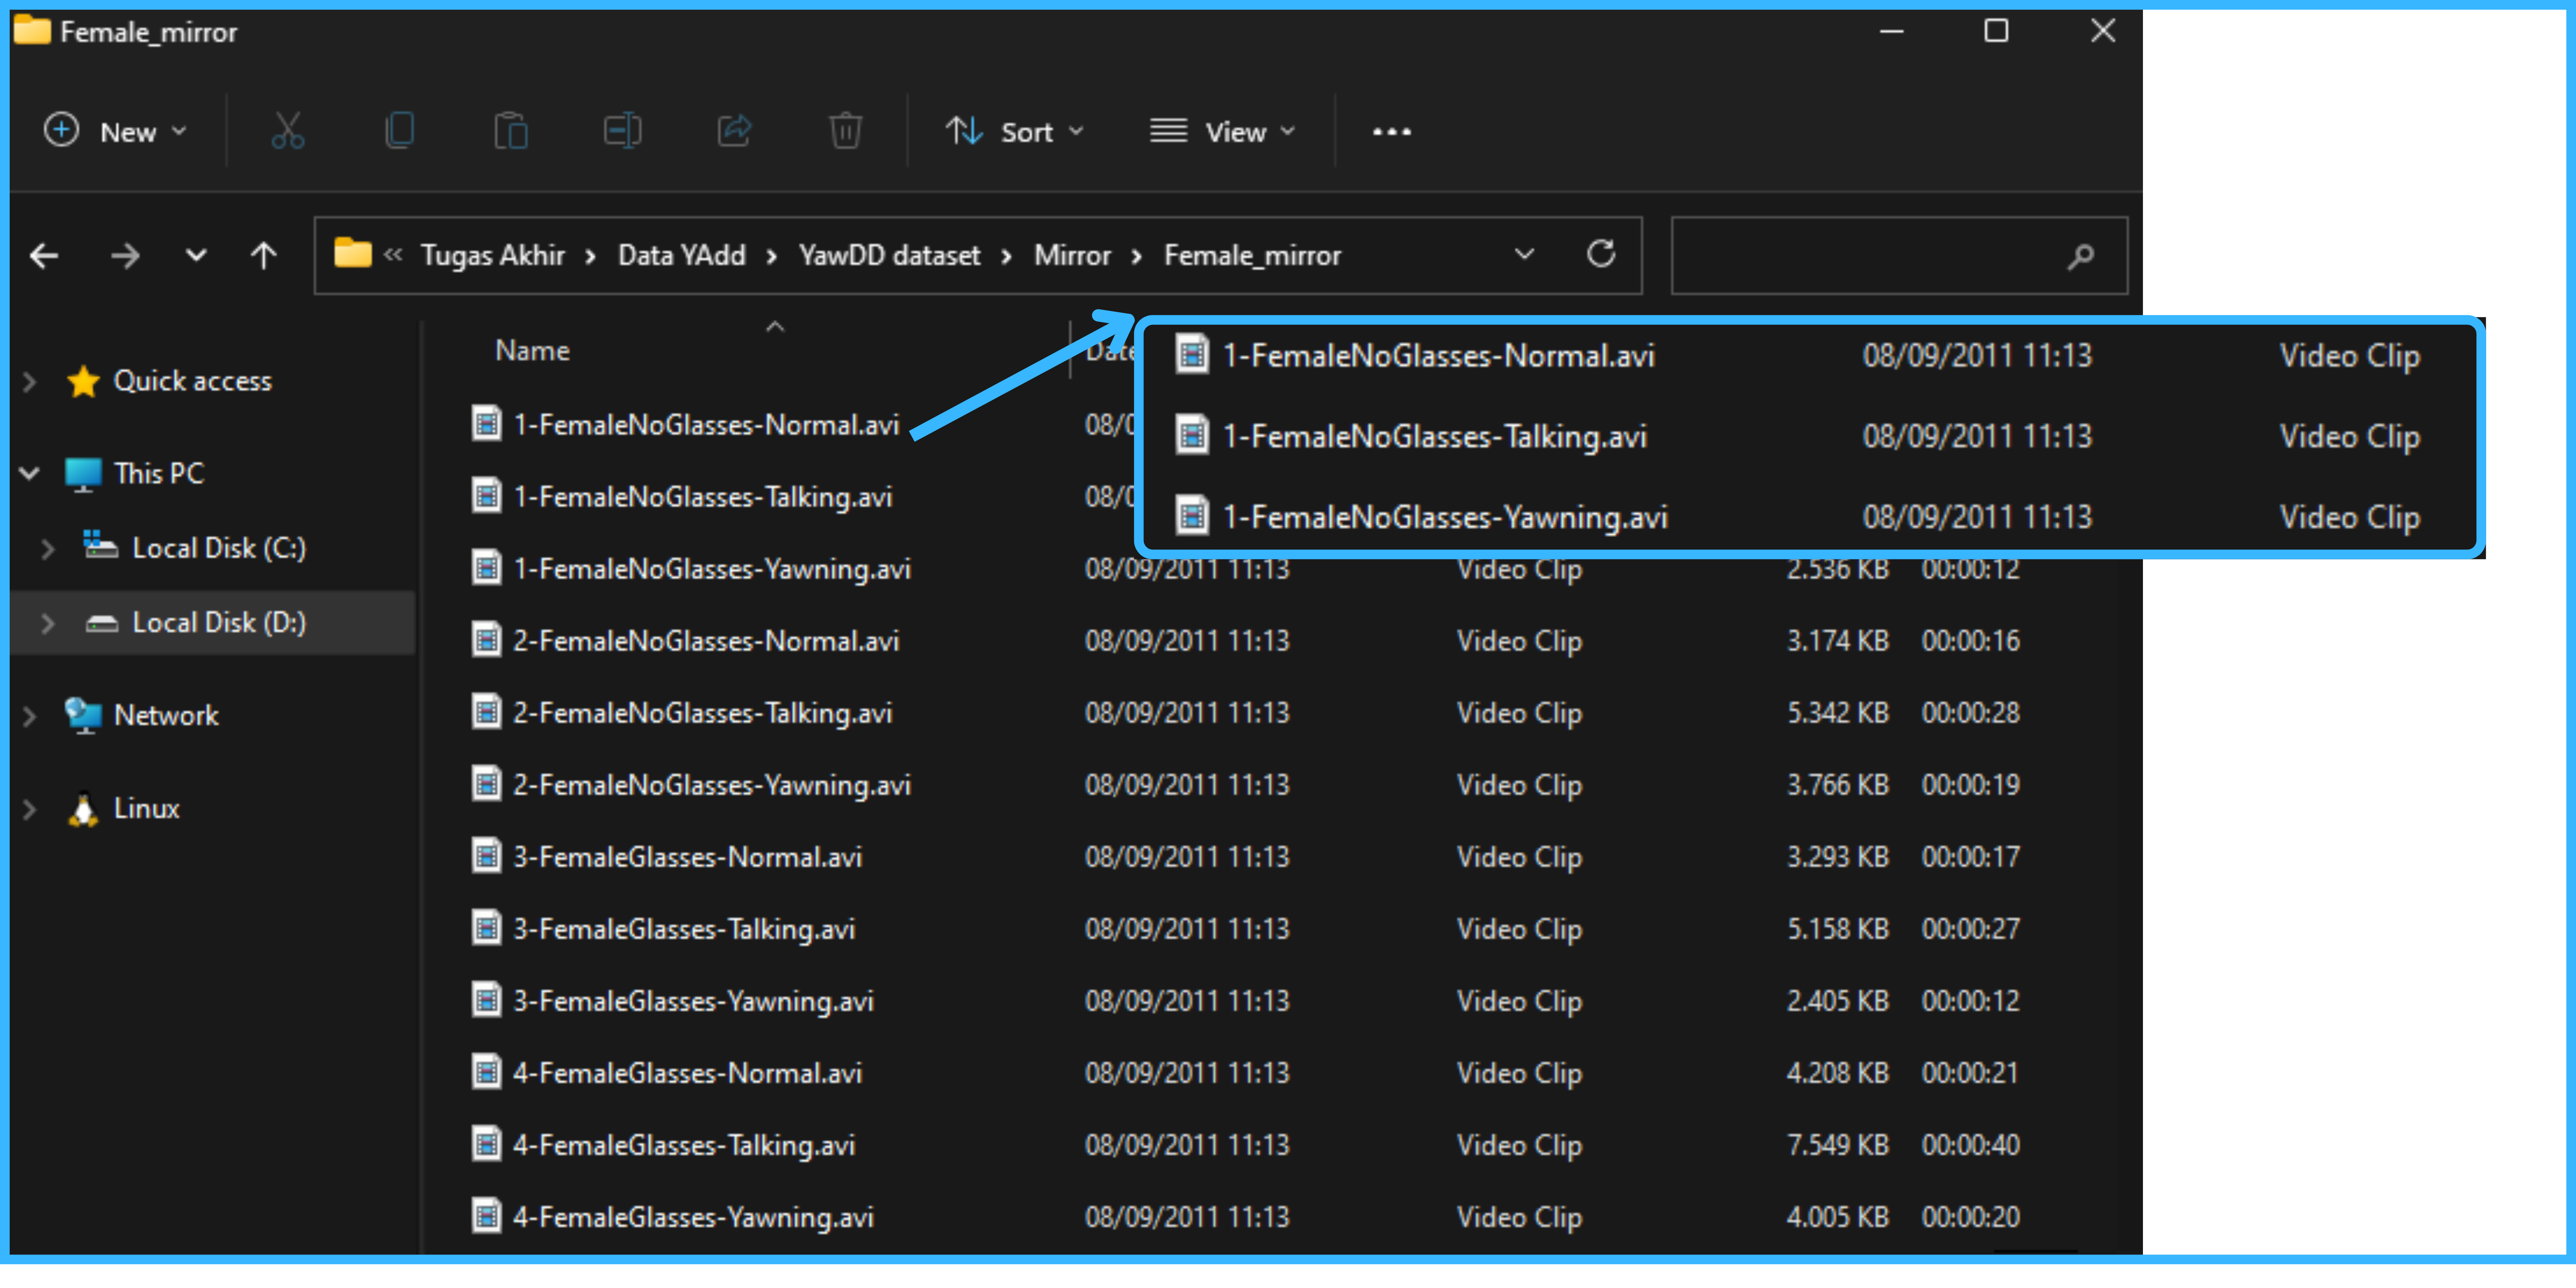
\includegraphics[width=\textwidth]{figures/bab4/seleksi_fitur.png}
             \caption{Seleksi Fitur}
             \label{Seleksi_Fitur}
     \end{figure}
   
   
   Pada penelitian ini, fokus diarahkan pada fitur \textit{'action}', hanya keadaan\textit{'yawning'} dan 
   \textit{'yawning \& talking'}  yang dipilih. Kondisi ini dipilih karena pengambilan data difokuskan pada pengemudi
    yang mengantuk dan menguap. Data kemudian diekstrak ke dalam format gambar (.jpg) dan dilatih pada model
     \textit{Convolutional Neural Network} (CNN). Seleksi data dilakukan berdasarkan dua kategori, yaitu data
      \textit{'male'}dan \textit{'female'}.

      Penelitian ini berfokus pada analisis fitur \textit{"action"} untuk mendeteksi rasa kantuk pada pengemudi. 
      Dari berbagai fitur \textit{"action"}, hanya dua keadaan yang dipilih, yaitu \textit{"yawning"} (menguap) dan
      \textit{"yawning \& talking"} (menguap dan berbicara). Pemilihan ini didasarkan pada fokus penelitian pada
        pengemudi yang menunjukkan tanda-tanda kantuk, seperti menguap. Data dikumpulkan dalam format 
        gambar (.jpg) dan kemudian dilatih menggunakan model \textit{Convolutional Neural Network} (CNN). 
        Proses seleksi data dilakukan berdasarkan dua kategori, yaitu \textit{"male"} (laki-laki) dan \textit{"female"}
         (perempuan).

\subsubsection{\textit{Male}}
          Sebelum proses seleksi data, dilakukan eksplorasi data awal terkait fitur-fitur pada data. Hal ini bertujuan untuk memahami karakteristik data dan meninjau kembali kelayakan fitur-fitur yang telah dipilih. Contoh data dengan kategori \textit{'male}' ditampilkan pada Gambar \ref{male gambar1} berikut.
       
     \begin{figure}[H]
         \centering
             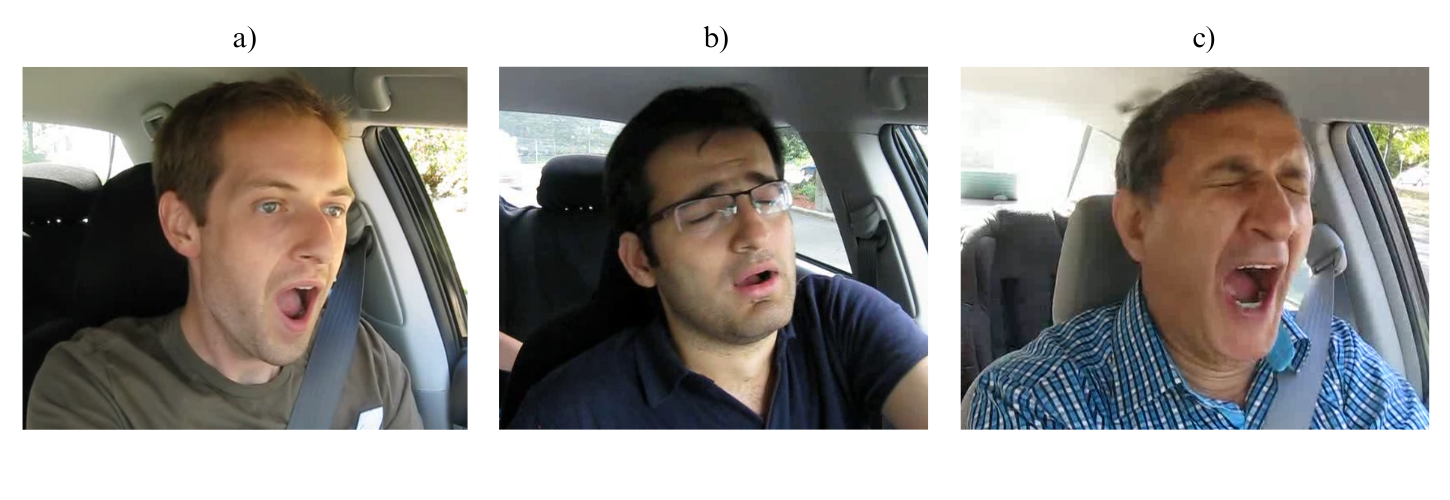
\includegraphics[width=\textwidth]{figures/bab4/male_contoh.png}
             \caption{Penampilan Data \textit{Male}}
             \label{male gambar1}
     \end{figure}

    Pada kategori data \textit{male} terdapat total 163 video (.avi). Berdasarkan deskripsi data pada fitur \textit{"action"} mencakup kondisi seperti \textit{"talking"}, \textit{"yawning"}, \textit{"normal"} dan \textit{"yawning \& talking"}. Proporsi data berdasarkan fitur \textit{action} pada kategori \textit{male} ditamilkan pada Gambar \ref{Proporsi Data Male Berdasarkan "Action"} berikut.
    

   

     \begin{figure}[H]
             \centering
         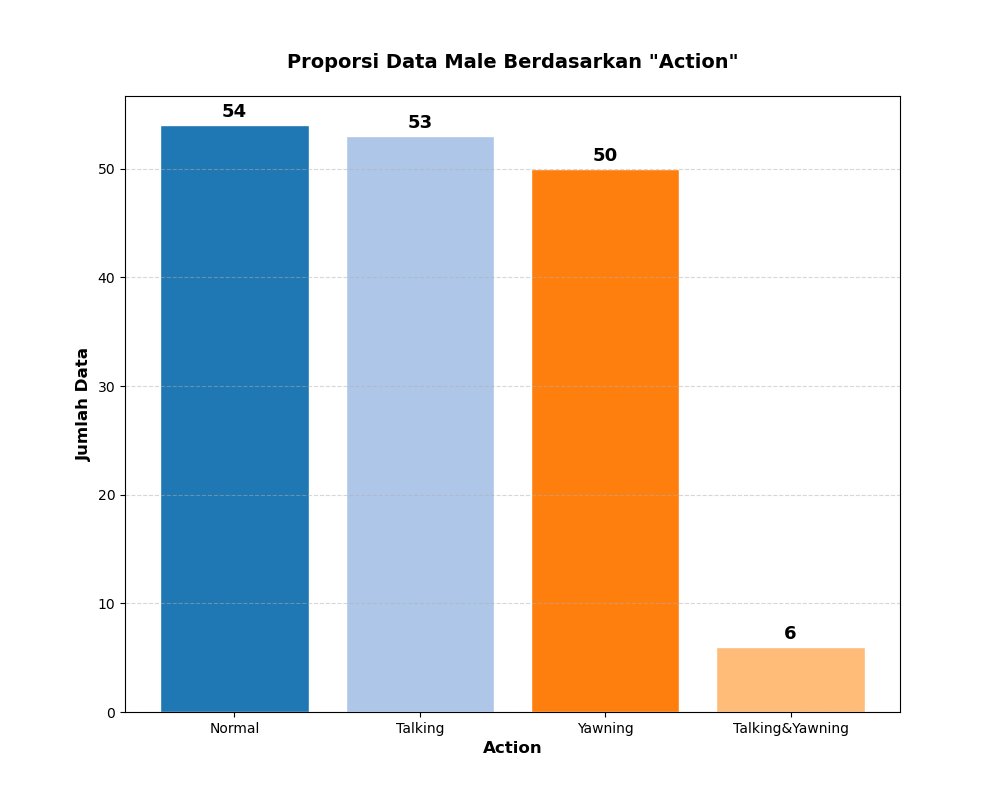
\includegraphics[width=0.75\linewidth]{figures/bab4/data_male.png}
         \caption{Proporsi Data \textit{Male} Berdasarkan \textit{"Action"}}
         \label{Proporsi Data Male Berdasarkan "Action"}
     \end{figure}

  


    Setelah dilakukan pemilihan fitur, di hasilkan jumlah data 
    untuk kategori \textit{male} sebanyak 56 video. Deskripsi untuk setiap data setelah sudah dilakukan pemilihan fitur untuk kategori \textit{male} ditampilkan pada Tabel \ref{Data male setelah dilakukan pemilihan fitur} berikut.

 
    \begin{table}[H]
        \centering
        \caption{Data \textit{Male} Setelah Dilakukan Pemilihan Fitur}
        \label{Data male setelah dilakukan pemilihan fitur}
        \scriptsize
        \begin{tabular}{p{0.2cm}p{1.2 cm}p{1.5cm}p{1.0cm}{0.5cm}{1.0 cm}{0.8 cm}{0.6cm}}
            \hline
            \textbf{No.} & \textbf{Participant Number} & \textbf{Action} & \textbf{Facial Hair} & \textbf{BG Movement} & \textbf{Glasses} & \textbf{Lighting} & \textbf{Ethnicity}\\
            \hline
            1 & 1 & Yawning & No & No & No Glasses & Sunny & Caucasian \\
            2 & 1 & Yawning & No & No & Sun glasses & Sunny & Caucasian \\
            3 & 2 & Yawning & No & Yes & Prescription & Sunny & Middle Eastern \\
            4 & 3 & Yawning & No & No & Prescription & Sunny & Caucasian  \\
            5 & 3 & Yawning & No & Yes & No Glasses & Sunny & Caucasian  \\
            6 & 4 & Yawning & No & No & No Glasses & Sunny & Middle Eastern  \\
            7 & 5 & Yawning & No & No & Sun glasses & Sunny & Middle Eastern  \\
            8 & 6 & Yawning & No & No & No Glasses & Sunny & Middle Eastern  \\
            9 & 7 & Yawning & No & No & Prescription & Sunny & Middle Eastern  \\
            10 & 8 & Yawning & Beard & Yes & Prescription & Sunny & Middle Eastern  \\
            11 & 9 & Yawning & No & No & No Glasses & Sunny & Caucasian \\
            12 & 10 & Yawning & No & No & No Glasses & Sunny & Middle Eastern  \\
            13 & 11 & Yawning & No & No & Prescription & Sunny & Middle Eastern \\
            14 & 12 & Talking \& Yawning & No & Yes & Prescription & Sunny & Middle Eastern  \\
            15 & 13 & Yawning & Beard & Yes & Prescription & Rainy & African  \\
            16 & 15 & Yawning & Beard & No & No Glasses & Rainy & African \\
            17 & 17 & Yawning & No & No & No Glasses & Sunny & Middle Eastern \\
            18 & 18 & Yawning & No & No & No Glasses & Sunny & Middle Eastern \\
            19 & 19 & Yawning & Moustache & No & Prescription & Sunny & Middle Eastern \\
            20 & 20 & Talking \& Yawning & No & No & Prescription & Sunny & Middle Eastern \\
            21 & 21 & Yawning & No & No & Prescription & Sunny & Middle Eastern \\
            22 & 22 & Yawning & Moustache & No & Prescription & Sunny & Middle Eastern \\
            23 & 23 & Talking \& Yawning & Beard & No & Prescription & Sunny & Middle Eastern  \\
            24 & 23 & Yawning & Beard & No & Prescription & Sunny & Middle Eastern  \\
            25 & 23 & Yawning & No & No & No Glasses & Sunny & Middle Eastern  \\
            26 & 24 & Yawning & No & No & Prescription & Cloudy & Middle Eastern \\
            27 & 25 & Yawning & Beard & No & Prescription & Cloudy & Middle Eastern  \\
            28 & 25 & Yawning & Beard & No & Sun glasses & Cloudy & Middle Eastern  \\
            29 & 26 & Yawning & No & Yes & No Glasses & Sunny & Middle Eastern \\
            30 & 27 & Yawning & No & No & Prescription & Sunny & Middle Eastern  \\
            31 & 27 & Yawning & No & No & No Glasses & Sunny & Middle Eastern  \\
            32 & 28 & Yawning & No & No & Prescription & Cloudy & Middle Eastern \\
            33 & 28 & Yawning & No & No & No Glasses & Cloudy & Middle Eastern \\
            34 & 29 & Yawning & No & Yes & No Glasses & Sunny & Caucasian  \\
            35 & 30 & Talking \& Yawning & No & Yes & Prescription & Sunny & Middle Eastern \\
            36 & 30 & Yawning & No & Yes & Prescription & Sunny & Middle Eastern  \\
            37 & 31 & Yawning & Beard & No & Prescription & Sunny & Middle Eastern  \\
            38 & 32 & Talking \& Yawning & No & Yes & Prescription & Cloudy & Middle Eastern \\
            39 & 32 & Yawning & No & No & Prescription & Cloudy & Middle Eastern \\
            40 & 33 & Talking \& Yawning & No & Yes & Prescription & Sunny & Middle Eastern \\
            41 & 33 & Yawning & No & No & Prescription & Sunny & Middle Eastern  \\
            42 & 34 & Yawning & No & Yes & No Glasses & Sunny & Caucasian \\
            43 & 35 & Yawning & No & No & No Glasses & Sunny & Middle Eastern \\
            44 & 36 & Yawning & No & Yes & No Glasses & Sunny & Caucasian  \\
            45 & 36 & Yawning & No & No & Sun glasses & Sunny & Caucasian \\
            46 & 37 & Yawning & Beard & Yes & No Glasses & Sunny & African  \\
            47 & 38 & Yawning & Beard & No & No Glasses & Sunny & African  \\
            48 & 38 & Yawning & Beard & Yes & Sun glasses & Sunny & African \\
            49 & 39 & Yawning & No & No & Prescription & Sunny & Asian & No \\
            50 & 40 & Yawning & No & No & No Glasses & Sunny & Middle Eastern  \\
            51 & 41 & Yawning & No & No & No Glasses & Sunny & Middle Eastern  \\
            52 & 42 & Yawning & No & No & No Glasses & Sunny & Middle Eastern  \\
            53 & 43 & Yawning & No & No & No Glasses & Sunny & Caucasian \\
            54 & 44 & Yawning & No & Yes & No Glasses & Sunny & Middle Eastern \\
            55 & 45 & Yawning & No & Yes & No Glasses & Sunny & Middle Eastern \\
            56 & 46 & Yawning & No & Yes & Prescription & Sunny & Middle Eastern \\
            \hline
        \end{tabular}
    \end{table}




\subsubsection{\textit{Female}}

    
    Pada kategori \textit{female} ditampilkan beberapa contoh data dengan kategori "\textit{female}" pada Gambar \ref{Female Dataset} berikut.
    
     \begin{figure}[H]
         \centering
         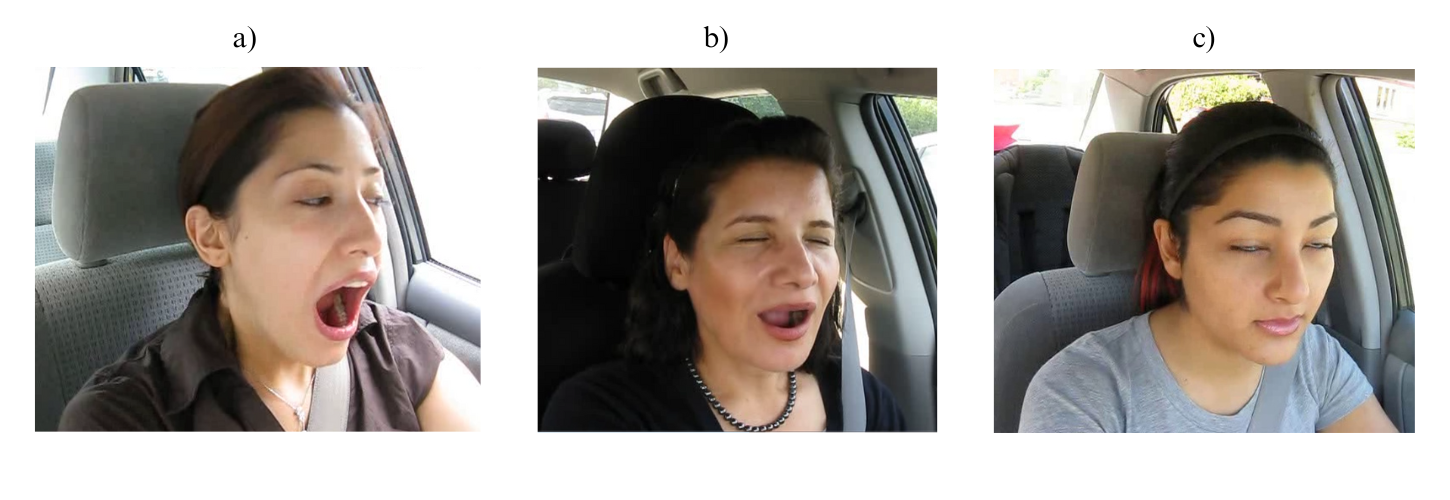
\includegraphics[width=1.0\linewidth]{figures/bab4/female_contoh.png}
         \caption{Contoh Data \textit{Female}}
         \label{Female Dataset}
     \end{figure}

   

     Terdapat 156 video pada kategori \textit{"female"}, fitur \textit{action} pada data mencakup keadaan \textit{"yawning"}, \textit{"talking"},\textit{"normal"} dan \textit{"yawning \& talking"}. Berikut proprosi untuk kategori \textit{action} di tampilkan pada Gambar \ref{Proporsi Data Female Berdasarkan "Action"} berikut.

     \begin{figure}[H]
         \centering
         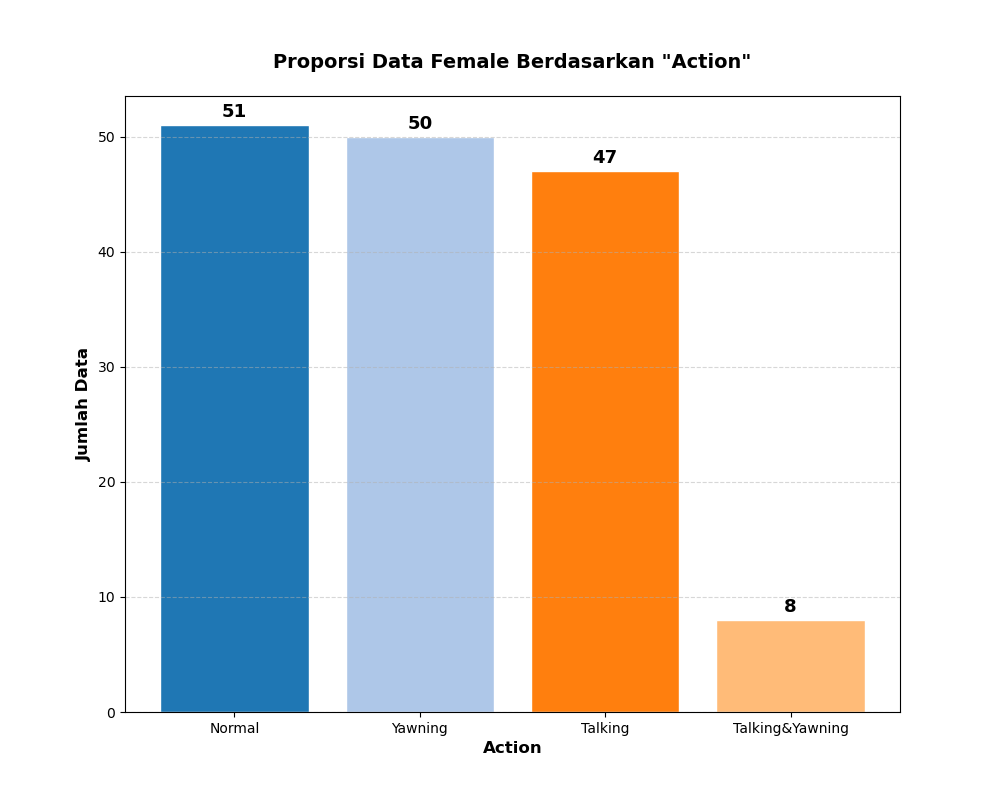
\includegraphics[width=0.75\linewidth]{figures/bab4/data_female.png}
         \caption{Proporsi Data \textit{Female }Berdasarkan \textit{"Action"}}
         \label{Proporsi Data Female Berdasarkan "Action"}
     \end{figure}

        Setelah dilakukan pemilihan fitur berdasarkan kolom 
        \textit{action}, yaitu hanya keadaan \textit{"yawning"} dan
         \textit{"talking \& yawning"} yang dipilih. Dihasilkan 
         jumlah data untuk kategori \textit{female} sebanyak 58 video. 
         Data \textit{female} setelah dilakukan pemilihan fitur 
         ditampilkan pada Tabel \ref{Data female setelah dilakukan pemilihan fitur} berikut.

        \begin{table}[H]
\centering
\caption{Data \textit{Female} Setelah Dilakukan Pemilihan Fitur}
\label{Data female setelah dilakukan pemilihan fitur}
\scriptsize

    \begin{tabular}{p{0.2cm}p{1.2 cm}p{1.5cm}p{1.0cm}{0.5cm}{1.0 cm}{0.8 cm}{0.6cm}}
    
    \hline
    \textbf{No.} & \textbf{Participant Number} & \textbf{Action} & \textbf{Scarf} & \textbf{BG Movement} & \textbf{Glasses} & \textbf{Lighting} & \textbf{Ethnicity} \\
    \hline
    1 & 2 & Yawning & No & No & No Glasses & Sunny & Middle Eastern \\
    2 & 5 & Yawning & No & No & No Glasses & Sunny & Middle Eastern  \\
    3 & 8 & Yawning & No & No & Prescription & Rainy & Caucasian  \\
    4 & 11 & Yawning & No & No & Prescription & Rainy & Caucasian \\
    5 & 14 & Yawning & No & No & Prescription & Rainy & Caucasian\\
    6 & 17 & Yawning & No & No & No Glasses & Rainy & Middle Eastern  \\
    7 & 20 & Yawning & No & No & Prescription & Cloudy & Middle Eastern \\
    8 & 23 & Yawning & No & No & Prescription & Cloudy & Middle Eastern  \\
    9 & 26 & Yawning & No & No & No Glasses & Cloudy & Middle Eastern \\
    10 & 29 & Yawning & No & No & No Glasses & Cloudy & Middle Eastern  \\
    11 & 32 & Yawning & No & Yes & No Glasses & Cloudy & Middle Eastern  \\
    12 & 35 & Yawning & No & Yes & No Glasses & Rainy & Middle Eastern \\
    13 & 38 & Talking \& Yawning & No & Yes & No Glasses & Sunny & Caucasian \\
    14 & 41 & Yawning & No & No & No Glasses & Sunny & Middle Eastern \\
    15 & 44 & Yawning & No & No & Prescription & Sunny & Middle Eastern  \\
    16 & 46 & Yawning & No & No & Sun glasses & Sunny & Middle Eastern  \\
    17 & 49 & Yawning & No & No & Prescription & Sunny & Middle Eastern \\
    18 & 52 & Yawning & No & No & No Glasses & Sunny & Middle Eastern \\
    19 & 55 & Yawning & No & No & Sun Glasses & Sunny & Middle Eastern  \\
    20 & 58 & Yawning & No & No & No Glasses & Sunny & Middle Eastern \\
    21 & 61 & Talking \& Yawning & No & No & Sun Glasses & Sunny & Middle Eastern  \\
    22 & 64 & Talking & No & No & No Glasses & Sunny & Middle Eastern  \\
    23 & 65 & Yawning & No & Yes & No Glasses & Sunny & Middle Eastern  \\
    24 & 68 & Yawning & No & Yes & No Glasses & Sunny & Middle Eastern \\
    25 & 71 & Yawning & Yes & No & No Glasses & Sunny & Middle Eastern  \\
    26 & 74 & Yawning & No & Yes & No Glasses & Sunny & Middle Eastern \\
    27 & 77 & Yawning & No & Yes & Sun Glasses & Cloudy & Middle Eastern \\
    28 & 79 & Talking & No & No & No Glasses & Cloudy & Middle Eastern  \\
    29 & 81 & Yawning & No & No & No Glasses & Cloudy & Middle Eastern  \\
    30 & 84 & Yawning & No & No & No Glasses & Sunny & Middle Eastern  \\
    31 & 86 & Yawning & No & No & No Glasses & Sunny & Caucasian  \\
    32 & 89 & Yawning & No & Yes & Sun glasses & Sunny & Caucasian \\
    33 & 92 & Yawning & No & No & Prescription & Sunny & Caucasian \\
    34 & 94 & Yawning & No & Yes & Sun glasses & Sunny & Caucasian  \\
    35 & 96 & Talking \& Yawning & No & No & No Glasses & Sunny & Caucasian \\
    36 & 99 & Yawning & No & No & Sun Glasses & Sunny & Caucasian  \\
    37 & 102 & Yawning & No & No & No Glasses & Sunny & Caucasian  \\
    38 & 105 & Yawning & No & No & No Glasses & Sunny & Middle Eastern  \\
    39 & 108 & Yawning & No & No & No Glasses & Sunny & Middle Eastern  \\
    40 & 111 & Yawning & No & Yes & Prescription & Cloudy & Asian  \\
    41 & 114 & Yawning & No & No & No Glasses & Cloudy & Asian  \\
    42 & 117 & Yawning & No & No & Sun Glasses & Cloudy & Middle Eastern \\
    43 & 120 & Yawning & No & Yes & No Glasses & Sunny & Middle Eastern \\
    44 & 122 & Talking \& Yawning & No & Yes & No Glasses & Sunny & Caucasian \\
    45 & 124 & Yawning & No & No & No Glasses & Sunny & Caucasian \\
    46 & 126 & Talking \& Yawning & No & No & No Glasses & Sunny & Middle Eastern \\
    47 & 128 & Yawning & No & Yes & No Glasses & Sunny & Middle Eastern  \\
    48 & 130 & Talking \& Yawning& No & Yes & No Glasses & Sunny & Middle Eastern  \\
    49 & 132 & Yawning & No & No & No Glasses & Sunny & Middle Eastern  \\
    50 & 134 & Talking \& Yawning& Yes & Yes & No Glasses & Sunny & Middle Eastern  \\
    51 & 136 & Yawning & Yes & No & No Glasses & Sunny & Middle Eastern  \\
    52 & 139 & Yawning & Yes & No & No Glasses & Sunny & Middle Eastern \\
    53 & 141 & Talking \& Yawning& No & Yes & No Glasses & Sunny & Middle Eastern  \\
    54 & 143 & Yawning & No & No & No Glasses & Sunny & Middle Eastern \\
    55 & 146 & Yawning & No & No & No Glasses & Sunny & Caucasian \\
    56 & 149 & Yawning & No & No & Prescription & Sunny & Middle Eastern  \\
    57 & 152 & Yawning & No & No & Sun Glasses & Sunny & Middle Eastern  \\
    58 & 155 & Yawning & No & No & No Glasses & Sunny & Middle Eastern \\
    \hline
\end{tabular}
\end{table}





    Setelah proses seleksi fitur, di mana hanya fitur
     \textit{"action"} dengan keadaan \textit{"yawning" }dan
      \textit{"yawning \& talking"} yang dipilih. Ditemukan sebanyak 58
       video untuk kategori \textit{"female"} dan sebanyak 56 video 
       untuk kategori \textit{"male"}. Dengan demikian, total data yang 
       diekstraksi menjadi gambar ada sebanyak 114 video.


\subsection{Penentuan Nilai EAR dan MAR}

    
    Nilai \textit{Eye Aspect Ratio} (EAR) dan 
    \textit{Mouth Aspect Ratio} (MAR) digunakan untuk 
    mengekstrak video menjadi format gambar (.jpg). 
    Nilai EAR dan MAR pada video yang berjumlah 114 hasil seleksi 
    fitur akan di visualisasikan menggunakan bantuan \textit{library} pada \textit{python} yaitu \textit{Open CV} dan \textit{Dlib}. Visualisasi ini bertujuan untuk melihat pola di angka berapa data tersebut mengantuk dan menguap. Keadaan mata kantuk dapat di lihat pada saat nilai EAR berada dibawah rata-rata dan menuju nilai nol. Keadaan menguap dapat dilihat pada saat nilai MAR berada diatas rata-rata. 
    
    Namun untuk menentukan ambang batas atau \textit{threshold} nilai MAR dan EAR dapat mendeteksi kantuk dan menguap dengan baik, dilakukan beberapa  percobaan pada nilai EAR dan MAR. Percobaan ini menggunakan 10 video yang diambil secara acak mewakili kategori \textit{male} dan \textit{female}. \textit{Eye Aspect Ratio} (EAR) dan \textit{Mouth Aspect Ratio} (MAR) yang memiliki nilai kesalahan terkecil akan digunakan untuk melakukan ekstraksi 114 video hasil seleksi fitur sebelumnya.

\subsubsection{\textit{Eye Aspect Ratio} (EAR)}

        
         \begin{figure}[H]
             \centering
             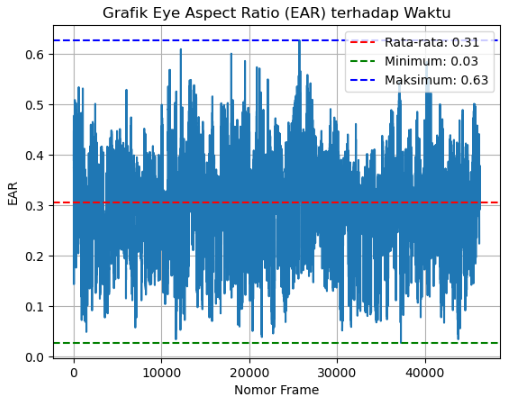
\includegraphics[width=0.75\linewidth]{figures/bab4/nilai ear.png}
             \caption{Grafik Nilai EAR}
             \label{Grafik Nilai EAR}
         \end{figure}

            Berdasarkan grafik pada Gambar \ref{Grafik Nilai EAR}, nilai EAR \textit{(Eye Aspect Ratio)} menunjukkan pola mengantuk berada dibawah rata-rata. Hal ini sesuai dengan teori yang menyatakan bahwa semakin kecil nilai EAR menunjukkan bahwa kondisi mata semakin tertutup. Namun perlu ditentukan ambang batas \textit{threshold} dimana nilai EAR menunjukkan mengantuk dengan kesalahan terkecil.
            
            Pada penentuan ambang batas tersebut akan dicoba ekstrak video dengan rentang nilai di bawah rata-rata yaitu $0.18 - 0.30$ dan diatas rata-rata yaitu $0.32 - 0.40$. Pemilihan rentang tersebut berdasarkan pola hasil visualisai nilai EAR yang menunjukkan pada rentang tersebut terdapat pola mata mengantuk. Selanjutnya akan di ekstrak video menjadi gambar kedalam dua kelas yaitu kantuk dan tidak kantuk. Tujuan mencoba bebera nilai ini untuk melihat di angka berapa nilai EAR dapat menentukan kantuk dan tidak kantuk dengan nilai kesalahan terkecil menggunakan Persamaan \ref{rumus error}. Nilai EAR yang dicoba untuk melakukan ekstraksi video menjadi gambar dapat di lihat pada Tabel \ref{Penentuan Nilai EAR} berikut.\\


            \begin{table}[h]
            \centering
            \caption{Eksperimen Penentuan Nilai EAR}
            \begin{tabular}{ccccc}
                \toprule
                 \textbf{No} &\textbf{Nilai EAR} & \textbf{Jumlah Kantuk} & \textbf{Salah Deteksi} & \textbf{\textit{Error (\%)}} \\
                \midrule
                   
                      
                         1 & 0.40 & 1863 & 1715 & 92.05 \\
                         2 &  0.38 & 1613 & 1465 & 90.82 \\
                         3 & 0.36 & 1332 & 1184 & 88.88 \\
                         4 &  0.34 & 1069 & 921  & 86.15 \\
                         5 &  0.32 & 796  & 648  & 81.00 \\
                         6 & \textbf{0.30} &\textbf{ 570} & \textbf{320} & \textbf{56.14} \\
                         7 & 0.28 & 400 & 220 & 55.00 \\
                         8 &  0.26 & 274 & 124 & 45.25 \\
                         9 &  0.24 & 196 & 104 & 53.06 \\
                         10 &  0.22 & 133 & 60& 45.11 \\
                         11 &  0.20 & 101 & 36  & 35.64 \\
                         12 &  0.18 & 87  & 30  & 34.48\\
    
                    \bottomrule
                \end{tabular}
                \label{Penentuan Nilai EAR}
            \end{table}

           Ekstraksi video dilakukan dengan cara membagi hasil setiap gambar menjadi dua kategori, yaitu kantuk dan tidak kantuk. Selanjutnya, dilakukan pemeriksaan kembali terhadap hasil ekstrak pada kategori kantuk untuk mengetahui jumlah sampel yang salah diklasifikasikan sebagai mengantuk, pada sesungguhnya tidak mengantuk. Hal ini dilakukan secara empiris atau melihat langsung hasil ekstraksi.


            Pada tabel \ref{Penentuan Nilai EAR} ditemukan bahwa nilai EAR yang berada di atas rata-rata memiliki nilai \textit{error} yang tinggi yaitu diatas angka $ 81\%$, hal ini menunjukkan bahwa nilai EAR diatas rata-rata tidak dapat mengelompokkan data dengan baik. Nilai \textit{error} di bawah rata-rata menunjukkan angkanya mengecil, hal ini menunjukkan semakin sedikitnya terjadi kesalahan prediksi. Visualisasi nilai EAR ditampilkan pada Gambar \ref{Eksperimen Penentuan Nilai EAR} berikut.

             \begin{figure}[H]
             \centering
                 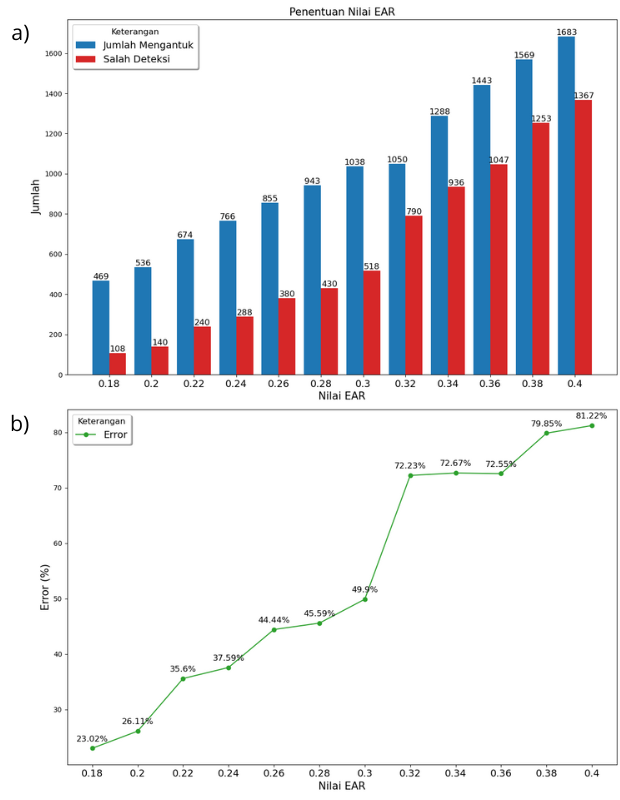
\includegraphics[width=0.8\textwidth]{figures/bab4/penentuan nilai ear.png}
                 \caption{a) Percobaan Nilai EAR, b) Nilai \textit{Error} EAR}
                 \label{Eksperimen Penentuan Nilai EAR}
             \end{figure}


          Dari hasil visualisasi pada Gambar \ref{Eksperimen Penentuan Nilai EAR} menunjukkan pola bahwa semakin besar nilai EAR jumlah yang terdeteksi kantuk juga semakin besar, namun nilai \textit{error }juga sangat kecil. Pola ini sesuai dengan teori yang menyatakan semakin kecil nilai EAR menunjukkan bahwa kondisi mata sedang tertutup atau mengantuk. Sehingga pada penentuan nilai EAR penelitian ini akan digunakan dengan nilai kesalahan atau \textit{error} yang terkecil yaitu dengan EAR sebesar 0.18 dengan \textit{error} sebesar $34.48\%$\\

    

\subsubsection{\textit{Mouth Aspect Ratio} (MAR)}
    
    
             \begin{figure}[H]
                 \centering
                 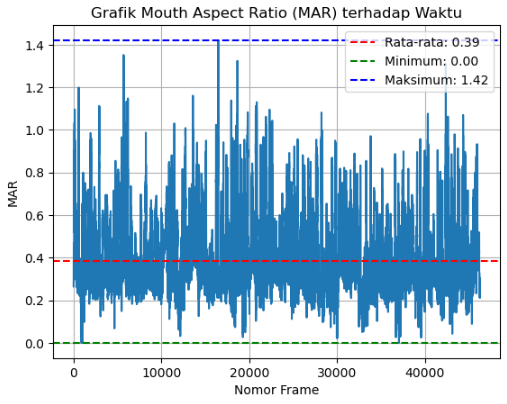
\includegraphics[width=0.8\linewidth]{figures/bab4/nilai mar.png}
                 \caption{Grafik Nilai MAR}
                 \label{Grafik Nilai MAR}
             \end{figure}



        
            Berdasarkan grafik pada Gambar \ref{Grafik Nilai MAR}, nilai MAR \textit{(Mouth Aspect Ratio)} menunjukkan pola menguap berada atas rata-rata. Hal ini sesuai dengan teori yang menyatakan bahwa semakin besar nilai MAR menunjukkan bahwa kondisi mulut semakin terbuka lebar. Namun perlu ditentukan ambang batas dimana nilai MAR menunjukkan keadaan menguap dengan kesalahan terkecil. Pada visualisasi menunjukkan bahwa berada pada rentang $0.00 - 1.42$ dengan minimum $0.00$ hingga maksimum $1.42$, dan rata-rata sebesar $0.39$. 
            
            Pada penentuan ambang batas akan dicoba ekstrak video dengan rentang nilai di bawah rata-rata yaitu $0.40 - 0.30$ dan diatas rata-rata yaitu $0.42 - 0.52$. Pemilihan rentang tersebut berdasarkan pola hasil visualisai nilai MAR yang menunjukkan pada rentang tersebut terdapat mulut terbuka dengan lebar. Selanjutnya akan di ekstrak video menjadi gambar kedalam dua kelas yaitu menguap dan tidak menguap. Tujuan mencoba bebera nilai ini untuk 
            melihat dan menentukan di angka berapa nilai MAR dapat mengklasifikasikan setiap gambar menguap dan tidak menguap dengan nilai kesalahan terkecil menggunakan Persamaan \ref{rumus error}. Cara ini serupa dilakukan seperti penentuan nilai EAR sebelumnya.
            
            Nilai MAR dan hasil percobaan untuk melakukan ekstraksi video menjadi gambar dapat di lihat pada Tabel \ref{Penentuan Nilai MAR} berikut.\\


        
            \begin{table}[h]
            \centering
            \caption{a) Percobaan Nilai MAR, b) Nilai \textit{Error} MAR}
            \begin{tabular}{ccccc}
                \toprule
                \textbf{No} &\textbf{Nilai MAR} & \textbf{Jumlah Menguap} & \textbf{Salah Deteksi} & \textbf{\textit{Error} (\%)} \\
                \midrule
                          1 & 0.30 & 1683 & 1367 &  81.22 \\
                          2 & 0.32 & 1569 & 1253 & 79.85 \\
                          3 & 0.34 & 1443 & 1047 & 72.55 \\
                          4 & 0.36 & 1288 & 936  & 72.67 \\
                          5 & 0.38 & 1050 & 790  & 75.23\\
                         6 & \textbf{0.40} & \textbf{1038}& \textbf{518} &  \textbf{49.90} \\
                          7 & 0.42 & 943 & 430 & 45.59 \\
                          8 & 0.44 & 855 & 380 & 44.44 \\
                          9 & 0.46 & 766 & 288 & 37.59 \\
                          10 & 0.48 & 674 & 240 & 35.60 \\
                          11 & 0.50 & 536 & 140  & 26.11 \\
                          12 & 0.52 & 469 & 108 & 23.02 \\
                         
                    \bottomrule
                \end{tabular}
                \label{Penentuan Nilai MAR}
            \end{table}


         %Visualisasi nilai MAR yang diuju dapat dilihat pada Gambar \ref{Eksperimen Penentuan Nilai MAR} berikut.

         \begin{figure}[H]
               \centering
               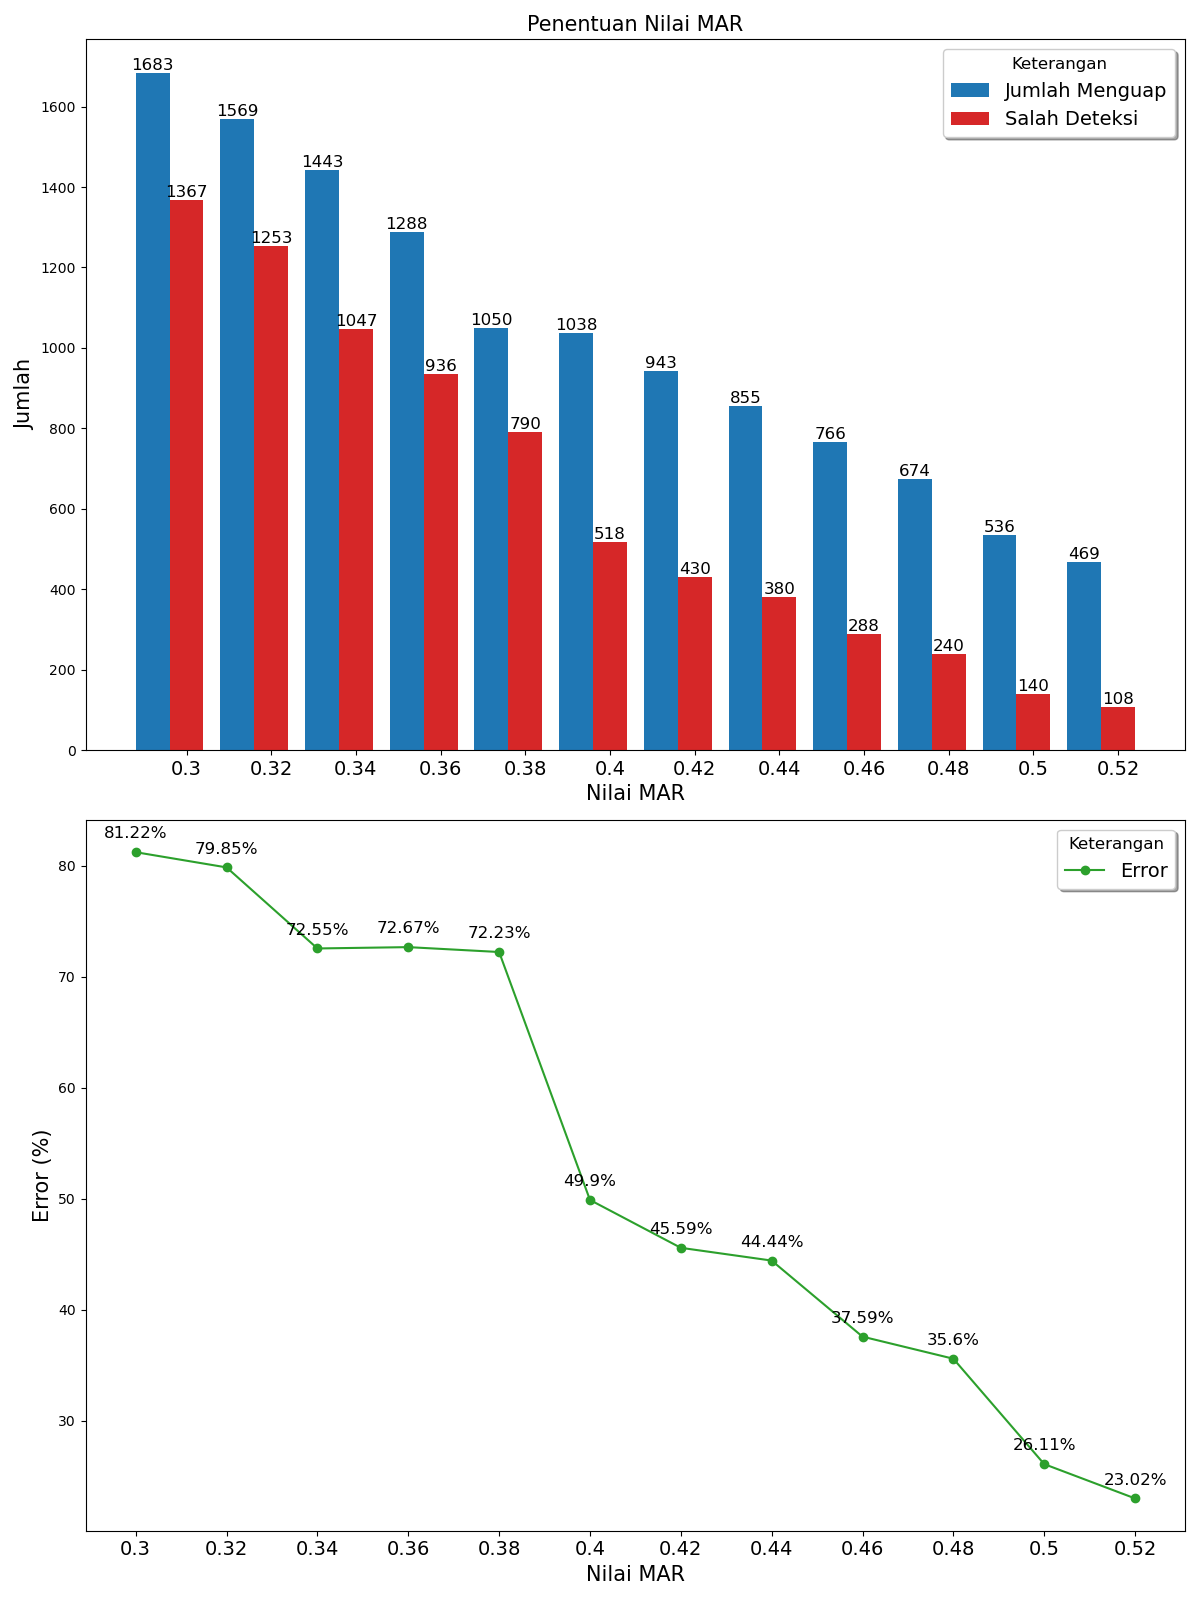
\includegraphics[width=0.8\textwidth]{figures/bab4/penentuan nilai mar.png}
               \caption{Eksperimen Penentuan Nilai MAR}
               \label{Eksperimen Penentuan Nilai MAR}

         \end{figure}

        Dari hasil visualisasi pada Gambar \ref{Eksperimen Penentuan Nilai MAR} menunjukkan pola bahwa semakin besar nilai MAR jumlah yang tereteksi 
        menguap juga semakin besar. Pola ini sesuai dengan teori yang menyatakan 
        semakin kecil nilai EAR menunjukkan bahwa kondisi mulut sedang terbuka lebar atau menguap. Sehingga pada penentuan nilai MAR penelitian ini akan digunakan dengan nilai kesalahan atau \textit{error} yang terkecil yaitu dengan MAR sebesar 0.52 dengan \textit{error} sebesar $23.02\%$\\



    Setelah dilakukan percobaan menggunakan beberapa nilai EAR (\textit{Eye Aspect Ratio}) dan MAR (\textit{Mouth Aspect Ratio}). Diperoleh nilai kesalahan terkecil untuk EAR sebesar 0.18 dan MAR 0.52. Kedua nilai ini digunakan untuk melakukan ekstraksi data secara keseluruhan.
    
\subsection{Ekstraksi Data}

     Setelah diperoleh nilai \textit{Eye Aspect Ratio }(EAR) dan \textit{Mouth Aspect Ratio} (MAR) 
     terbaik dengan nilai \textit{error} terkecil. Selanjutnya dilakukan ektraksi data secara keseluruhan 
     dari bentuk bentuk video (.avi) ke format gambar (.jpg). Data di ekstrak menjadi tiga kelas 
     yaitu "mengantuk \& menguap", "mengantuk \& tidak menguap", "menguap \& tidak mengantuk". 
     Proses ekstrak video agar menghasilkan data dengan format gambar sesuai dengan kelas yang 
     ditentukan dilakukan dengan kondisi seperti Gambar \ref{kondisi ear dan mar} berikut.


              \begin{figure}[H]
              \caption{Kondisi Penentuan Nilai EAR dan MAR}
               \centering
               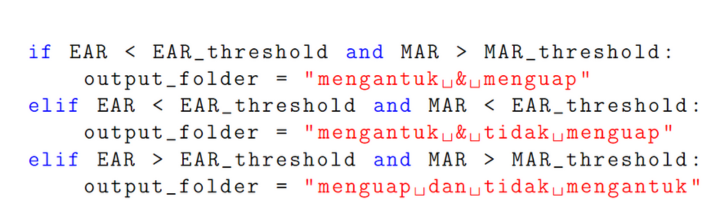
\includegraphics[width=0.90\textwidth]{figures/bab4/threshold.png}
               \caption{Pembagian Data}
               \label{kondisi ear dan mar}

         \end{figure}

     
   
    
    
    Setiap foto hasil ektraksi akan langsung otomatis masuk kedalam folder sesuai dengan kelas yang telah ditentukan. Pada ektraksi nilai \textit{thereshold} untuk EAR sebesar 0.18 dan nilai \textit{thereshold} MAR sebesar 0.58 kedua nilai ini diperoleh dari nilai terbaik hasil percobaan sebelumnya.

    \begin{enumerate}
        \item    Jika nilai EAR pada \textit{frame} tersebut lebih kecil dari EAR \textit{threshold} dan MAR lebih besar MAR \textit{threshold} foto akan masuk dalam folder "mengantuk \& menguap".

        \item Jika nilai EAR pada \textit{frame} tersebut lebih kecil dari EAR \textit{threshold} dan MAR lebih kecil
    dari MAR \textit{threshold} foto akan masuk dalam folder "mengantuk \& tidak menguap "


     \item  Jika nilai EAR pada \textit{frame} tersebut lebih besar dari EAR \textit{threshold} dan MAR lebih besar
    dari MAR \textit{threshold} foto akan masuk dalam folder "menguap \& tidak mengantuk"

    
        

    \end{enumerate}
    

     
     Hasil ekstrak data video menjadi gambar ditampilkan pada tabel \ref{Hasil Ekstraksi Data} berikut. 

       \begin{table}[H]
            \centering
            \caption{Hasil Ekstraksi Data}
            \begin{tabular}{cc}
                \toprule
                \textbf{Kelas} & \textbf{Hasil Ekstrak} \\
                \midrule  
                           Mengantuk dan Menguap & 1038  \\
                          Mengantuk tidak Menguap & 1304 \\
                           Menguap tidak Mengantuk& 2042  \\
                
                    \bottomrule
                \end{tabular}
                \label{Hasil Ekstraksi Data}
            \end{table}

        Pada tabel \ref{Hasil Ekstraksi Data} Ditemukan jumlah hasil ekstraksi untuk kelas "mengantuk dan menguap" 
        berjumlah 1038 gambar, "mengantuk dan tidak menguap" berjumlah 1304 gambar dan kelas yang terakhir
         "menguap tidak mengantuk" berjumlah 2042 gambar. Kondisi ini menunjukkan bahwa hasil ekstraksi 
         data pada setiap kelasnya \textit{imbalance}, hal ini dapat mempengaruhi hasil akurasi saat 
         dilakukan klasifikasi dengan CNN. Selanjutnya, untuk memperkaya jumlah data dan mengatasi 
         data \textit{imbalance} atau tidak seimbang pada setiap kelasnya dilakukan teknik augmentasi data. 
         Augmentasi data yang diterapkan adalah seperti \textit{zoom}, \textit{grayscal}e dan \textit{shear} 
         dengan metode \textit{oversampling} dengan konfigurasi seperti Tabel \ref{Perlakuan Augmentasi Data} berikut.

        
\begin{table}[H]
    \centering
    \caption{Perlakuan Augmentasi Data}
    \label{Perlakuan Augmentasi Data}
    \begin{tabular}{
        >{\raggedright\arraybackslash}p{1.0cm} 
        >{\raggedright\arraybackslash}p{2.5cm} 
        >{\raggedright\arraybackslash}p{9.3cm}}
        \hline
        \textbf{No} & \textbf{Augmentasi} & \textbf{Tujuan} \\
        \hline
        1 & \textit{zoom} & Memperbesar ukuran gambar dengan skala tertentu, nilai skala \textit{zoom} yang digunakan sebesar 0.3 atau 30\% dari gambar asli \\
        2 & \textit{sheer} & Melakukan transformasi yang memiringkan gambar ke arah tertentu, nilai \textit{shear} yang digunakan sebesar 90 derajat \\
        3 & \textit{grayscle} & Mengubah  gambar menjadi warna abu-abu atau hitam putih \\
        
        \hline
    \end{tabular}
\end{table}

     
        
        Hal ini bertujuan untuk membuat distribusi kelas menjadi seimbang. Augmentasi dilakukan dengan melakukan satu perlakukan untuk satu data pada jumlah kelas tertinggi. Kemudian jumlah ini menjadi acuan untuk kelas lainnya dengan maksimal data yang di augmentasi sebanyak jumlah data pada jumlah data kelas tertinggi. Sehingga pada masukan model CNN data menjadi seimbang. Jumlah data sebelum dan sesudah dilakukan augmentasi ditampilkan pada Tabel \ref{Hasil Augmentasi Data} berikut.
    


            \begin{table}[H]
            \centering
            \caption{Hasil Ekstraksi Data}
            \begin{tabular}{ccc}
                \toprule
                \textbf{Kelas} & \textbf{Hasil Ekstrak} & \textbf{Augmentasi }\\
                \midrule
                      
                           Mengantuk dan Menguap & 1038 & 4084 \\
                          Mengantuk tidak Menguap & 1304 & 4084 \\
                           Menguap tidak mengantuk& 2042 & 4084 \\
                
                    \bottomrule
                \end{tabular}
                \label{Hasil Augmentasi Data}
            \end{table}




    
    \subsection{Pembagian Data}
    
    Sebelum data dilatih, dilakukan pembagian data menjadi data 
    \textit{train} dan data \textit{test}. Pembagian data ini 
    dilakukan dengan menggunakan metode \textit{KFold Cross Validation}. 
    Teknik ini melibatkan pembagian data menjadi beberapa \textit{subset}. 
    Menerapkan pembagian data dengan \textit{KFold Cross Validation} 
    bertujuan untuk mencegah \textit{overfitting}, 
    menghasilkan estimasi performa model yang stabil, 
    membandingkan model, dan memperkirakan generalisasi model. 
    Dengan hal ini dapat memperoleh perkiraan kinerja model yang 
    lebih akurat dan membantu dalam pemilihan model terbaik pada 
    saat \textit{training} dilakukan. 
    
    Peneliti menerapkan \textit{fold} sebesar lima untuk mempekecil waktu komputasi. Sehingga keseluruhan data dibagi menjadi lima lipatan dan dilatih sebanyak lima kali berdasarkan jumlah \textit{fold }yang telah ditentukan sebelumnya. Pembagian data diilustrasikan seperti pada Gambar \ref{Pembagian Data} berikut.

         \begin{figure}[H]
               \centering
               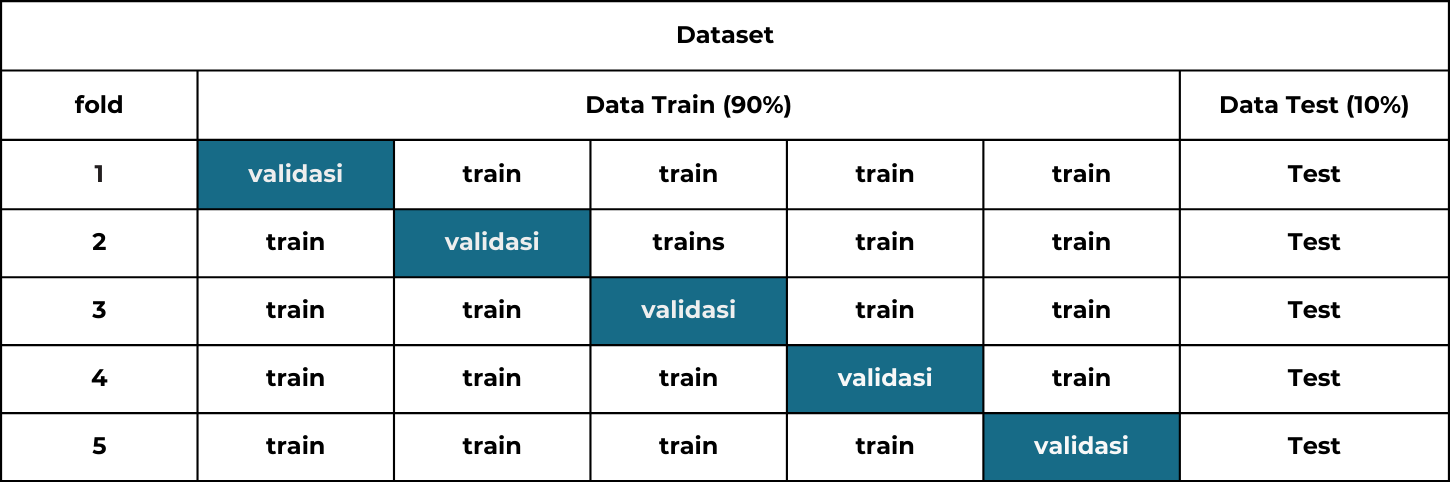
\includegraphics[width=0.90\textwidth]{figures/bab4/kfold.png}
               \caption{Pembagian Data}
               \label{Pembagian Data}

         \end{figure}



    Dari keseluruhan data hasil ekstraksi dan augmentasi diperoleh jumlah data sebanyak 12.252 gambar, 10\% dari keselurahan data dibagi menjadi data \textit{test} yaitu sebanyak 1227 gambar. Pada data \textit{test} jumlah data untuk setiap kelasnya sama yaitu sebanyak 409 gambar. Untuk data 90\% dibagi berdasarkan jumlah \textit{KFold} yang telah ditetapkan yaitu $k = 5$, sehingga diperoleh untuk setiap \textit{foldnya} berjumlah sebanyak 2205 gambar dengan jumlah data setiap data kelasnya seimbang.
    



\section{Arsitektur CNN}

    Arsitektur CNN yang digunakan memiliki \textit{input shape} sebesar $ 64 x 64 $ piksel dan terdapat beberapa \textit{layer} yang digunakan dalam pembuatan model untuk melakukan klasifikasi. Berikut adalah ringkasan arsitektur yang digunakan:

    \begin{enumerate}
        \item     \textit{Convolutional Layers}: Terdapat tiga blok \textit{convolutional layer} yang masing-masing terdiri dari dua \textit{layer} Conv2D dengan aktivasi ReLU dan \textit{padding} yang sama. Blok pertama memiliki 32 filter, blok kedua memiliki 64 filter, dan blok ketiga memiliki 128 filter.
    
        \item  \textit{Batch Normalization}: Dilakukan setelah setiap blok \textit{convolutional }untuk mempercepat proses konvergensi dan mengurangi \textit{overfitting}.
    
        \item \textit{Max Pooling Layers}: Setelah setiap blok \textit{convolutional}, dilakukan \textit{max pooling} dengan ukuran sebesar (2,2) untuk mengurangi dimensi gambar.
    
       \item  \textit{Dropout}: Setelah \textit{max pooling} terakhir, dilakukan \textit{dropout} dengan nilai 0.2 untuk mengurangi \textit{overfitting}.
    
        \item \textit{Flatten Layer}: Digunakan untuk mengubah \textit{output} dari \textit{layer} sebelumnya menjadi vektor satu dimensi.
    
        \item \textit{Dense Layers:} Terdapat dua \textit{layer dense} setelah \textit{flatten layer}. \textit{Layer} pertama memiliki 256 unit dengan aktivasi ReLU dan \textit{layer} terakhir memiliki tiga unit dengan aktivasi \textit{softmax}, sesuai dengan jumlah kelas yang ada.

    \end{enumerate}

    Untuk desain arsitektur \textit{Convolutional Neural Network} (CNN) yang digunakan ditampilkan pada Tabel 
    \ref{Desain arsitektur} berikut.

    

    \begin{table}[H]
        \centering
        \scriptsize
        \caption{Desain Arsitektur}
        \label{Desain arsitektur}
        \renewcommand{\arraystretch}{1.5}
        \begin{tabular}{p{1cm}p{4.5cm}p{4cm}p{2.5cm}}
        \hline
        \textbf{No} & \textbf{Layer (type)}   & \textbf{Output Shape} & \textbf{Parameters}  \\ \hline
        
        1 & conv2d                   & (64, 64, 32)   & 896     \\ 
        2 & conv2d\_1                & (64, 64, 32)   & 9248    \\ 
        3 & batch\_normalization     & (64, 64, 32)   & 128     \\ 
        4 & max\_pooling2d           & (32, 32, 32)   & 0       \\ 
        5 & conv2d\_2                & (32, 32, 64)   & 18496   \\ 
        6 & conv2d\_3                & (32, 32, 64)   & 36928   \\ 
        7 & batch\_normalization\_1  & (32, 32, 64)   & 256     \\ 
        8 & max\_pooling2d\_1        & (16, 16, 64)   & 0       \\ 
        9 & conv2d\_4                & (16, 16, 128)  & 73856   \\ 
        10 & conv2d\_5                & (16, 16, 128)  & 147584  \\ 
        11 & batch\_normalization\_2  & (16, 16, 128)  & 512     \\ 
        12 & max\_pooling2d\_2        & (8, 8, 128)    & 0       \\ 
        13 & dropout                  & (8, 8, 128)    & 0       \\ 
        14 & flatten                  & (8192)         & 0       \\ 
        15 & dense                    & (256)          & 2097408 \\ 
        16 & dense\_1                 & (3)            & 771     \\ \hline
        \end{tabular}
    \end{table}





\section{Pengujian Model CNN}

    Dalam rangka menguji model, beberapa skenario dijalankan untuk mengidentifikasi model terbaik.
     Penelitian ini menguji beberapa parameter, sebagaimana dijelaskan pada Tabel \ref{Pengujian Parameter}, dengan 
     tujuan untuk menentukan parameter optimal.  Akurasi \textit{test} yang dimaksud pada pengujian 
     ini adalah menggunakan data validasi, sedangkan \textit{activation function} yang digunakan 
     hanya pada \textit{hidden layer}.


    
        
\subsection{Pengujian \textit{Learning Rate} dan \textit{Activation Layer}}

    Pada pengujian ini menampilkan evaluasi dari \textit{accuracy} \textit{train}, \textit{validation} \textit{train}, \textit{test}, \textit{precision}, \textit{recall} dan \textit{F1-Score}.

\subsubsection{\textit{Learning Rate} 0.01}

        \begin{table}[H]
        \centering
        \caption{Pengujian \textit{Learning Rate} 0.01 }
        \begin{tabular}{ccccc}
            \toprule
            \multicolumn{5}{c}{\textit{Learning Rate} 0.01} \\ \hline
            
            \textbf{\textit{Activation}} & \multicolumn{1}{c}{\textbf{\textit{KFold}}} & \textbf{\textit{Train Acc (\%)} } & \textbf{\textit{Val Acc (\%)}} & \textbf{\textit{Test Acc (\%)}}  \\
    
            \midrule
            \multirow{5}{*}{ReLU} 
            & 1 & 48.19 & 48.48 & 54.42  \\
            & 2 & 67.88 & 62.13 & 63.08 \\
            & 3 & 51.34 & 46.77 & 51.81 \\
            & 4 & 32.68 & 33.93 & 35.29 \\
            & 5 & 36.14 & 33.39 & 45.91 \\ 
            & \textbf{\textit{mean}}& \textbf{47.24 }& \textbf{44.94} & \textbf{50.10} \\ \hline

    
            \multirow{5}{*}{Sigmoid}
            & 1 & 33.46 & 33.56 & 33.83  \\
            & 2 & 33.97 & 34.14 & 34.14 \\
            & 3 & 33.12 & 32.57 & 34.34 \\
            & 4 & 34.24 & 32.84 & 34.16 \\
            & 5 & 34.03 & 33.12 & 33.75 \\
            & \textit{\textbf{mean}}& \textbf{33.76} & \textbf{33.24} &\textbf{34.04} \\ 
                        \hline
    
            \multirow{5}{*}{Softmax}
            & 1 & 33.10 & 32.47 & 33.92 \\
            & 2 & 33.63 & 32.97 & 33.51 \\
            & 3 & 33.10 & 33.12 & 34.21  \\
            & 4 & 33.27 & 32.66 & 33.71 \\
            & 5 & 33.38 & 32.94 & 33.80 \\
            & \textit{\textbf{mean}}& \textbf{33.29} & \textbf{32.83} &\textbf{33.83} \\ 
    

            \bottomrule
            \end{tabular}
            \label{Pengujian Learning Rate 0.01 }
        \end{table}

    Pengujian fungsi \textit{activation function} dengan \textit{learning rate} 0.01 
    pada ReLU diperoleh rata-rata akurasi untuk \textit{training} sebesar 47.24\%, validasi sebesar 44.94\% dan test sebesar 50.10\%. Namun akurasi model cukup bervariasi di setiap iterasi \textit{KFold}, dapat dilihat pada akurasi \textit{training} diperoleh nilai terkecil sebesar 32.68\% dan terbesar 67.88\%.
    Hal ini menunjukkan bahwa model sensitif terhadap pembagian data. Pada \textit{activation function} \textit{sigmoid} diperoleh rata-rata akurasi untuk \textit{training} sebesar 33.76\%, validasi sebesar 33.24\% dan test sebesar 34.04\%. Akurasi pada \textit{sigmoid} stabil di setiap iterasi \textit{KFold} tapi akurasi yang dihasilkan jauh lebih kecil jika dibandingkan dengan ReLU.
    
    Pada \textit{activation function} \textit{softmax} akurasi rata-rata untuk \textit{training} sebesar 33.29\%, validasi sebesar 33.83\% dan test sebesar 33.83\%. Akurasi pada \textit{softmax} juga stabil di setiap iterasi \textit{KFold} tapi akurasi yang dihasilkan lebih kecil jika dibandingkan dengan ReLU dan \textit{sigmoid}. Pada pengujian \textit{activation function} untuk \textit{learning rate} 0.01 \textit{activation function} terbaik adalah ReLU dengan rata-rata akurasi untuk \textit{training} sebesar 47.24\%, validasi sebesar 44.94\% dan test sebesar 50.10\%.

    

        \begin{table}[H]
        \centering
        \caption{Evaluasi \textit{Learning Rate} 0.01}
        \begin{tabular}{ccccc}
            \toprule
            \multicolumn{5}{c}{\textit{Learning Rate} 0.01} \\ \hline
            
            \textbf{\textit{Activation}} & \multicolumn{1}{c}{\textbf{\textit{KFold}}} & \textbf{\textit{Precision (\%)} } & \textbf{\textit{Recall (\%)}} & \textbf{\textit{F1-Score (\%)}}  \\
    
            \midrule
            \multirow{5}{*}{ReLU} 

            & 1 & 81.54 & 54.42 & 63.25  \\
            & 2 & 76.90 & 63.08 & 65.95 \\
            & 3 & 82.63 & 51.81 & 62.80\\
            & 4 & 91.16 & 35.29 & 48.00\\
            & 5 & 80.00 & 45.91 & 54.39 \\ 
            & \textbf{\textit{mean}}& \textbf{82.44} & \textbf{50.10} & \textbf{58.87} \\ \hline
            
            \multirow{5}{*}{Sigmoid}
            & 1 &  33.33 & 33.83 & 50.55  \\
            & 2 &  33.33  & 34.14 & 50.59 \\
            & 3 &  33.33  & 34.34 & 51.13 \\
            & 4 &  33.33  & 34.16 & 50.92 \\
            & 5 &  33.33  & 33.75 & 50.47 \\
            & \textit{\textbf{mean}}& \textbf{33.33} & \textbf{34.04} &\textbf{50.73} \\ 
                        \hline
    
            \multirow{5}{*}{Softmax}
            & 1 & 33.33  & 33.92 & 50.66 \\
            & 2 & 33.33  & 33.51 & 50.20 \\
            & 3 & 33.33  & 34.21 & 50.98  \\
            & 4 & 33.33  & 33.71 & 50.42 \\
            & 5 & 33.33  & 33.80 & 50.52 \\
            & \textit{\textbf{mean}}& \textbf{33.33} & \textbf{33.83} &\textbf{50.55} \\ 
    

            \bottomrule
        \end{tabular}
        \label{Evaluasi Learning Rate 0.01 }
    \end{table}

      Evaluasi model pada \textit{activation function} dengan \textit{learning rate} 0.01 menunjukkan bahwa \textit{activation function} \textit{ReLU} menghasilkan nilai rata-rata \textit{precision} sebesar 82,44\%, \textit{recall} 50,10\%, dan\textit{ F1-Score} 58,87\%. Hal ini menunjukkan kecenderungan \textit{activation function} \textit{ReLU} untuk memprioritaskan prediksi positif daripada mengidentifikasi semua contoh positif. Hal ini terlihat dari nilai \textit{precision} yang jauh lebih tinggi dibandingkan \textit{recall}.

     Pada \textit{activation function} \textit{sigmoid} diperoleh nilai rata-rata pada \textit{precision} sebesar 33.33\%, \textit{recall} sebsar 34.04\% dan\textit{ F1-Score} sebesar 50.73\%. Hasil untuk \textit{sigmoid} menunjukkan bahwa model hanya dapat memprediksi satu kelas saja, hal ini dapat di lihat pada nilai \textit{precision} yang sama setiap iterasi KFold. Pada \textit{activation function} \textit{softmax} diperoleh nilai rata-rata pada \textit{precision} sebesar 33.33\%, \textit{recall} sebesar 33.83\% dan \textit{F1-Score} sebesar 50.55\%.
     Berdasarkan hasil evaluasi, \textit{activation function} ReLU menghasilkan performa terbaik dengan 
     rata-rata \textit{F1-Score} tertinggi. \textit{Sigmoid} dan \textit{softmax} memiliki performa yang jauh lebih rendah dan perlu dioptimalkan lebih lanjut.


 

    \subsubsection{\textit{Learning Rate} 0.001}
    
    \begin{table}[H]
        \centering
        \caption{Pengujian \textit{Learning Rate} 0.001 }
        \begin{tabular}{ccccc}
            \toprule
            \multicolumn{5}{c}{\textit{Learning Rate} 0.001} \\ \hline
            
            \textbf{\textit{Activation}} & \multicolumn{1}{c}{\textbf{\textit{KFold}}} & \textbf{\textit{Train Acc (\%)} } & \textbf{\textit{Val Acc (\%)}} & \textbf{\textit{Test Acc (\%)}}  \\
    
            \midrule
            \multirow{5}{*}{ReLU} 
            & 1 & 91.41 & 86.98 & 90.70  \\
            & 2 & 90.84 & 86.12 & 91.84 \\
            & 3 & 89.42 & 80.49 & 87.70 \\
            & 4 & 91.10 & 90.79 & 92.24 \\
            & 5 & 91.99 & 90.42 & 91.74  \\
            & \textit{\textbf{mean}}& \textbf{90.95} & \textbf{86.96} &\textbf{ 90.84} \\ \hline
    
            \multirow{5}{*}{Sigmoid}
            & 1 &  93.72 & 65.17 & 87.30  \\
            & 2 &  91.15 & 47.21 & 69.52 \\
            & 3 &  89.24 & 60.93 & 86.25 \\
            & 4 &  33.56 & 32.98 & 34.16 \\
            & 5 &  59.35 & 40.01 & 46.23 \\
            & \textit{\textbf{mean}}& \textbf{73.40} & \textbf{49.26} &\textbf{64.69} \\ 
                        \hline
    
            \multirow{5}{*}{Softmax}
            & 1 & 32.99 & 31.79 & 34.28 \\
            & 2 & 33.27 & 33.65 & 33.65 \\
            & 3 & 33.04 & 32.35 & 34.93  \\
            & 4 & 33.18 & 32.57 & 33.93 \\
            & 5 & 33.20 & 32.94 & 32.94 \\
            & \textit{\textbf{mean}}& \textbf{33.13} & \textbf{32.66} &\textbf{33.94} \\ 

            \bottomrule
        \end{tabular}
        \label{Pengujian Learning Rate 0.001}
    \end{table}

    Pengujian \textit{activation function} untuk \textit{learning rate} 0.001 
    pada \textit{ReLU} diperoleh rata-rata akurasi untuk \textit{training} sebesar 91.41\%, validasi sebesar 86.96\% dan test sebesar 90.84\%. Pada \textit{learning rate} 0.001 terjadi peningkatan akurasi yang signifikan dari akurasi menggunakan \textit{learning rate} 0.01. Sebelumnya hanya diperoleh rata-rata akurasi untuk \textit{training} sebesar 47.24\%, validasi sebesar 44.94\% dan test sebesar 50.10\%. Pada \textit{learning rate} 0.001 juga diperoleh akurasi setiap iterasi \textit{KFold} jauh lebih stabil dibandingkan sebelumnya. 

    \textit{Activation function} \textit{sigmoid} memiliki akurasi rata-rata untuk \textit{training} sebesar 73.40\%, validasi sebesar 49.26\% dan test sebesar 64.69\%. Penggunaan \textit{learning rate} 0.001 untuk \textit{activation function} \textit{sigmoid} juga mengalami peningkatan yang tinggi dari sebelumnya rata-rata akurasi untuk \textit{training} sebesar 33.33\%, validasi sebesar 34.04\% dan test sebesar 50.73\%. Namun pada setiap iterasi \textit{KFold} akurasi sangat tidak stabil hal ini dibuktikan terdapat akurasi tertinggi sebesar 93.72\% dan terendah sebesar 33.56\%. Hal ini menunjukkan pembagian data sangat sensitif pada \textit{activation function} sigmoid. Pada \textit{activation function} \textit{softmax} memiliki akurasi rata-rata untuk \textit{training} sebesar 33.13\%, validasi sebesar 32.66\% dan test sebesar 33.94\%. Pada \textit{softmax} tidak ada perubahan yang cukup signifikan dari penggunaan \textit{learning rate} sebelumnya. 

     Penurunan \textit{learning rate} dari 0.01 ke 0.001 menunjukkan pengaruh yang signifikan terhadap kinerja \textit{activation function} \textit{ReLU} dan \textit{sigmoid}. Namun pada perubahan \textit{learning rate} tidak menunjukkan efek yang substansial pada \textit{activation function} \textit{softmax}.
    
    
    
    

   

    \begin{table}[H]
        \centering
        \caption{Evaluasi \textit{Learning Rate} 0.001 }
        \begin{tabular}{ccccc}
            \toprule
            \multicolumn{5}{c}{\textit{Learning Rate} 0.001} \\ \hline
            
            \textbf{\textit{Activation}} & \multicolumn{1}{c}{\textbf{\textit{KFold}}} & \textbf{\textit{Precision (\%)} } & \textbf{\textit{Recall (\%)}} & \textbf{\textit{F1-Score (\%)}}  \\
    
            \midrule
            \multirow{5}{*}{ReLU} 

            & 1 & 91.89 & 90.70 & 90.80  \\
            & 2 & 92.04 & 91.83 & 91.80 \\
            & 3 & 87.82 & 87.70 & 87.72\\
            & 4 & 92.20 & 92.24 & 92.21\\
            & 5 & 91.68 & 91.74 & 91.70 \\
            & \textit{\textbf{mean }} & \textbf{91.12} & \textbf{90.84} & \textbf{90.84 }\\ \hline

            
            \multirow{5}{*}{Sigmoid}
            & 1 & 88.20 & 87.30 & 87.20  \\
            & 2 & 83.43 & 69.52 & 73.23 \\
            & 3 & 86.43 & 86.25 & 86.09 \\
            & 4 & 100.00 & 34.16 & 50.92 \\
            & 5 & 72.05 & 46.23 & 55.97 \\
            & \textit{\textbf{mean}}& \textbf{86.02} & \textbf{64.69} &\textbf{70.68} \\ 
                        \hline
    
            \multirow{5}{*}{Softmax}
            & 1 & 33.33  & 34.28 & 51.06 \\
            & 2 & 33.33  & 33.65 & 50.35 \\
            & 3 & 33.33  & 34.93 & 51.78  \\
            & 4 & 33.33  & 33.93 & 50.67 \\
            & 5 & 33.33  & 32.94 & 49.55 \\
            & \textit{\textbf{mean}}& \textbf{33.33} & \textbf{33.94} &\textbf{50.68} \\ 
    

            \bottomrule
        \end{tabular}
        \label{Evaluasi Learning Rate 0.001 }
    \end{table} 

\vspace{1cm}


    Evaluasi model untuk \textit{activation function} dengan \textit{learning rate} 0.001 menunjukkan bahwa \textit{activation function} \textit{ReLU} menghasilkan nilai rata-rata \textit{precision} sebesar 91.12\%, \textit{recall} 90.84\%, dan \textit{ F1-Score} 90.84\%. Hasil ini jauh lebih baik dari pada penggunaan \textit{learning rate} 0.01 karena nilai rata-rata yang lebih tinggi dan untuk setiap metriks yang dihasilkan juga stabil. 
    
     Pada \textit{activation function}\textit{sigmoid} diperoleh nilai rata-rata pada \textit{precision} sebesar 86.02\%, \textit{recall} sebsar 64.69\% dan\textit{ F1-Score} sebesar 70.68\%. Hasil pada \textit{sigmoid} menunjukkan perubahaan \textit{learning rate} menjadi 0.01 cukup berarti, hal ini dibuktikan adanya peningkatan nilai pada setiap mariks evaluasi. Sementara pada \textit{activation function} \textit{softmax} diperoleh nilai rata-rata pada \textit{precision} sebesar 33.33\%, \textit{recall} sebsar 33.94\% dan\textit{ F1-Score} sebesar 50.68\%.
     Perubahan \textit{learning rate} pada \textit{activation function} \textit{sigmoid} tidak memiliki hasil yang berarti. 
     
     Pada penggunaan \textit{learning rate} 0.001 hasil evaluasi menunjukkan \textit{activation function} terbaik diperoleh pada ReLU nilai \textit{ F1-Score} 90.84\%.
     
  

    

   \subsubsection{\textit{Learning Rate} 0.0001} 

   
        \begin{table}[H]
        \centering
        \caption{Pengujian \textit{Learning Rate} 0.0001 }
        \begin{tabular}{ccccc}
            \toprule
            \multicolumn{5}{c}{\textit{Learning Rate} 0.0001} \\ \hline
            
            \textbf{\textit{Activation}} & \multicolumn{1}{c}{\textbf{\textit{KFold}}} & \textbf{\textit{Train Acc (\%)} } & \textbf{\textit{Val Acc (\%)}} & \textbf{\textit{Test Acc (\%)}}  \\
    
            \midrule
            \multirow{5}{*}{ReLU} 

            & 1 & 90.46 & 87.02 & 91.88 \\
            & 2 & 93.00 & 89.02 & 91.97 \\
            & 3 & 97.25 & 83.03 & 90.29 \\
            & 4 & 90.22 & 89.11 & 90.69 \\
            & 5 & 93.02 & 92.00 & 93.69 \\ 
            & \textit{\textbf{mean}}& \textbf{92.79} & \textbf{88.03} &\textbf{91.70.} \\ 
            \hline


            \multirow{5}{*}{Sigmoid}
            & 1 &  84.93 & 69.75 & 76.73  \\
            & 2 &  71.23 & 41.40 & 69.43 \\
            & 3 &  68.32 & 35.34 & 63.15 \\
            & 4 &  71.27 & 57.89 & 70.37 \\
            & 5 &  65.51 & 37.47 & 46.09 \\
            & \textit{\textbf{mean}}& \textbf{72.25} & \textbf{48.37} &\textbf{65.15} \\ 
                        \hline
    
            \multirow{5}{*}{Softmax}
            & 1 & 33.71 & 31.79 & 31.79 \\
            & 2 & 33.01 & 33.24 & 33.24 \\
            & 3 & 33.01 & 32.71 & 32.71  \\
            & 4 & 32.92 & 33.48 & 33.48 \\
            & 5 & 33.43 & 32.94 & 32.94 \\
            & \textit{\textbf{mean}}& \textbf{33.21} & \textbf{32.83} &\textbf{32.83} \\ 

            \bottomrule
        \end{tabular}
        \label{Pengujian Learning Rate 0.0001 }
    \end{table}

    Pengujian \textit{activation function} untuk \textit{learning rate} 0.0001 
    pada \textit{ReLU} diperoleh rata-rata akurasi untuk \textit{training} sebesar 92.79\%, validasi sebesar 88.03\% dan test sebesar 91.70\%. Pada \textit{learning rate} 0.0001 terjadi peningkatan akurasi sekitar dua persen dari penggunaan \textit{learning rate} 0.001. 
    
    Penggunaan \textit{activation function} \textit{sigmoid} memiliki akurasi rata-rata untuk \textit{training} sebesar 72.25\%, validasi sebesar 48.37\% dan test sebesar 65.15\%. Penggunaan \textit{learning rate} 0.0001 untuk \textit{activation function} \textit{sigmoid} tidak terdapat pola peningkatan akurasi malah mengalami penurunan akurasi sekitar satu persen. Pada hasil ini menunjukkan bahwa penurunan nilai \textit{learning rate} pada \textit{activation function} \textit{sigmoid}
    tidak selalu mengalami peningkatan akurasi. 

    Pada \textit{activation function} \textit{softmax} memiliki akurasi rata-rata untuk \textit{training} sebesar 33.21\%, validasi sebesar 32.83\% dan test sebesar 32.83\%. Hasil \textit{activation function} \textit{sofmaxt} tidak mengalami perubahan yang begitu besar dari penggunaan \textit{learning rate} 0.0001, 0.001, 0.01, Sehingga dapat disimpulkan pengaruh \textit{learning rate} untuk \textit{softmax }tidak cukup berpengaruh.



    \begin{table}[H]
        \centering
        \caption{Evaluasi \textit{Learning Rate} 0.0001 }
        \begin{tabular}{ccccc}
            \toprule
            \multicolumn{5}{c}{\textit{Learning Rate} 0.0001} \\ \hline
            
            \textbf{\textit{Activation}} & \multicolumn{1}{c}{\textbf{\textit{KFold}}} & \textbf{\textit{Precision (\%)} } & \textbf{\textit{Recall (\%)}} & \textbf{\textit{F1-Score (\%)}}  \\
    
            \midrule
            \multirow{5}{*}{ReLU} 
            
            & 1 & 92.09 & 91.88 & 91.87 \\
            & 2 & 92.28 & 91.97 & 91.95 \\
            & 3 & 91.11 & 90.29 & 90.35 \\
            & 4 & 90.77 & 90.69 & 90.70 \\
            & 5 & 93.84 & 93.69 & 93.71 \\ 
            & \textit{\textbf{mean}}& \textbf{91.01} & \textbf{91.70} &\textbf{91.71} \\ 
            \hline


            
            \multirow{5}{*}{Sigmoid}
            & 1 &  82.05 & 76.73 & 77.49  \\
            & 2 &  70.47 & 69.43 & 69.65 \\
            & 3 &  71.52 & 63.15 & 65.22  \\
            & 4 &  70.94 & 70.37 & 70.51 \\
            & 5 &  72.78 & 46.09 & 51.60 \\
            & \textit{\textbf{mean}}& \textbf{73.55} & \textbf{65.15} &\textbf{66.89} \\ 
                        \hline
    
            \multirow{5}{*}{Softmax}
            & 1 & 33.33  & 31.79 & 48.24 \\
            & 2 & 33.33  & 33.24 & 49.89 \\
            & 3 & 33.33  & 32.71 & 49.29 \\
            & 4 & 33.33  & 33.48 & 50.16 \\
            & 5 & 33.33  & 32.94 & 49.55 \\
            & \textit{\textbf{mean}}& \textbf{33.33} & \textbf{32.83} &\textbf{49.42} \\ 
    

            \bottomrule
        \end{tabular}
        \label{Evaluasi Learning Rate 0.0001 }
    \end{table}

      Evaluasi model pada \textit{activation function} dengan \textit{learning rate} 0.0001 \textit{activation function} \textit{ReLU} menghasilkan nilai rata-rata \textit{precision} sebesar 91.01\%, \textit{recall} 91.70\%, dan\textit{ F1-Score} 91.71\%. Pada 
      Penggunaan \textit{learning rate} 0.0001 hasil prediksi setiap kelasnya cukup stabil di bandingkan sebelumnya. 
      
      Pada \textit{activation function} \textit{sigmoid} diperoleh nilai rata-rata pada \textit{precision} sebesar 73.55\%, \textit{recall} sebsar 65.15\% dan\textit{ F1-Score} sebesar 66.89\%. Hasil untuk \textit{sigmoid} menunjukkan lebih rendah dengan penggunaan \textit{learning rate} 0.001 yaitu dengan nilai rata-rata pada \textit{precision} sebesar 86.02\%, \textit{recall} sebsar 64.69\% dan\textit{ F1-Score} sebesar 70.68\%. Sementara pada \textit{activation function} \textit{softmax} diperoleh nilai rata-rata pada \textit{precision} sebesar 33.33\%, \textit{recall} sebsar 32.83\% dan\textit{ F1-Score} sebesar 49.42\%.
     Perubahan \textit{learning rate} pada \textit{activation function} \textit{softmax} tidak memiliki perubahan yang berarti. 
     
     
     
    Pengujian dan evaluasi \textit{activation function} \textit{ReLU, sigmoid dan sigmoid} pada \textit{learning rate} 0.0001, 0.001, 0.01 diperoleh hasil yang terbaik pada \textit{activation function} \textit{ReLU} dengan \textit{learning rate} 0.0001. \textit{activation function} ini menghasilkan nilai rata-rata  akurasi untuk \textit{training} sebesar 92.79\%, validasi sebesar 88.03\% dan test sebesar 91.70\%, \textit{precision} sebesar 91.01\%, \textit{recall} 91.70\%, dan\textit{ F1-Score} 91.71\%.

\subsection{Pengujian \textit{Optmizer}}

    Parameter \textit{learning rate} dan \textit{activation function} terbaik yang dihasilkan, akan digunakan mencari \textit{optimizer} terbaik dengan membandingkan fungsi optimasi \textit{Stochastic Gradient Descent} (SGD) dan \textit{Adaptive Moment Estimation} (Adam). Hasil dari pengujian ditampilkan pada Tabel \ref{Pengujian Optimizer} berikut.

        \begin{table}[H]
        \centering
        \caption{Pengujian \textit{Optimizer}}
        \begin{tabular}{ccccc}
            \toprule
            \textbf{\textit{Optimizer}} & \multicolumn{1}{c}{\textbf{KFold}} & \textbf{\textit{Train Acc (\%) } } & \textbf{\textit{Val Acc (\%)}} & \textbf{\textit{Test Acc (\%)}}\\
        
            \midrule
            \multirow{5}{*}{Adam} 
            & 1 & 90.46 & 87.02 & 91.88 \\
            & 2 & 93.00 & 89.02 & 91.97 \\
            & 3 & 97.25 & 83.03 & 90.29 \\
            & 4 & 90.22 & 89.11 & 90.69 \\
            & 5 & 93.02 & 92.00 & 93.69 \\ 
            & \textit{\textbf{mean}}& \textbf{92.79} & \textbf{88.03} &\textbf{91.70.} \\ 
            \hline

    
            \multirow{5}{*}{SGD}
            & 1 & 92.85 & 90.74 & 94.78 \\
            & 2 & 91.64 & 91.64 & 93.24 \\
            & 3 & 91.61 & 91.78 & 91.78 \\
            & 4 & 91.07 & 92.96 & 92.96 \\
            & 5 & 91.65 & 92.10 & 92.10  \\
            & \textit{\textbf{mean}}& \textbf{91.74} & \textbf{91.84} &\textbf{92.97} \\ 
    

            \bottomrule
        \end{tabular}
        \label{Pengujian Optimizer}
    \end{table}


    Setelah dilakukan pengujian \textit{optimizer} dan membandingkan 
    hasil \textit{Stochastic Gradient Descent} (SGD) 
     \textit{Adaptive Moment Estimation} (Adam). 
     Pada Adam diperoleh rata-rata akurasi \textit{training} 
     sebesar 92.79\%, validasi sebesar 88.03\% dan test sebesar 91.70\%. 
     Jika dibandingkan dengan SGD yaitu \textit{training} sebesar 91.74\%, 
     validasi sebesar 91.84\% dan test sebesar 92.97\%. Pada 
      \textit{training} Adam lebih unggul dibandingkan dengan 
       sebesar 1.05\% namun SGD lebih stabil dan konsisten pada 
        iterasi \textit{KFold} dan akurasi validasi dan test pada SGD
         juga lebih tinggi dari pada Adam.
    

        \begin{table}[H]
        \centering
        \caption{Evaluasi \textit{Optimizer}}
        \begin{tabular}{ccccc}
            \toprule
            \textbf{\textit{Optimizer}} & \multicolumn{1}{c}{\textbf{KFold}} & \textbf{\textit{Precision (\%) } } & \textbf{\textit{Recall (\%)}} & \textbf{\textit{F1-Score (\%)}}\\
        
            \midrule
            \multirow{5}{*}{Adam} 
            & 1 & 92.09 & 91.88 & 91.87 \\
            & 2 & 92.28 & 91.97 & 91.95 \\
            & 3 & 91.11 & 90.29 & 90.35 \\
            & 4 & 90.77 & 90.69 & 90.70 \\
            & 5 & 93.84 & 93.69 & 93.71 \\ 
            & \textit{\textbf{mean}}& \textbf{91.01} & \textbf{91.70} &\textbf{91.71} \\ 
            \hline

    
            \multirow{5}{*}{SGD}
            & 1 & 94.94 & 94.78 & 94.78 \\
            & 2 & 93.22 & 93.24 & 93.22 \\
            & 3 & 93.41 & 91.78 & 91.99 \\
            & 4 & 92.97 & 92.96 & 92.90 \\
            & 5 & 92.08 & 92.10 & 92.04  \\
            & \textit{\textbf{mean}}& \textbf{93.32} & \textbf{92.72} &\textbf{92.98} \\ 
    

            \bottomrule
        \end{tabular}
        \label{Evaluasi Optimizer}
    \end{table}

    Evaluasi model yang membandingkan \textit{optimizer} \textit{Stochastic Gradient Descent} (SGD) dan
     \textit{Adaptive Moment Estimation} (Adam).  \textit{Adam} menghasilkan nilai rata-rata \textit{precision} 
     sebesar 91.01\%, \textit{recall} 91.70\%, dan\textit{ F1-Score} 91.71\%. SGD lebih unggul dari setiap 
     matriks dengan selisih satu persen dari Adam. Nilai rata-rata \textit{precision} sebesar 93.32\%, 
     \textit{recall} 92.72\%, dan\textit{ F1-Score} 92.78\%. \textit{Optimizer} SGD lebih stabil di setiap KFold dibandingkan Adam karena pembaruan parameter yang konsisten, 
     generalisasi lebih baik, dan pengaturan parameter yang lebih sederhana. Adam, meskipun konvergensi lebih cepat, 
     sering mengalami variabilitas dan ketidakstabilan karena penyesuaian learning rate adaptif dan
      \textit{hyperparameter} yang lebih banyak.

    


    Dari semua hasil percobaan yang telah dilakukan ditampilakn ringkasan rata-rata dari hasil matriks penilaian pada Tabel \ref{Ringkasan Hasil Percobaan} berikut.


\begin{table}[H]
    \centering
    \caption{Ringkasan Hasil Percobaan}
    \begin{tabular}{ccccccc}
        \toprule
        \multirow{2}{*}{\textbf{\textit{Rate}}} & \multirow{2}{*}{\textbf{\textit{Activation}}} & \multirow{2}{*}{\textbf{\textit{Optimizer}}} & \multicolumn{3}{c}{\textbf{\textit{Metrics}}} \\
        \cmidrule{4-7}
        & & & \textbf{\textit{Accuracy}} & \textbf{\textit{Precision}} & \textbf{\textit{Recall}} & \textbf{\textit{F1-Score}} \\
        & & & \textbf{\textit{(\%)}} & \textbf{\textit{(\%)}} & \textbf{\textit{(\%)}} & \textbf{\textit{(\%)}} \\
        \midrule
        0.01 & ReLU   & Adam  & 50.10 & 82.24 & 50.10 & 58.87\\
        0.01 & Sigmoid & Adam  & 34.04 & 33.33 & 34.04 & 50.73 \\
        0.01 & Softmax & Adam  & 33.83 & 33.33 & 33.83 & 50.55\\
        \midrule
        0.001 & ReLU    & Adam  & 90.84 & 91.12 & 90.84 & 90.84\\
        0.001 & Sigmoid & Adam  & 64.69 & 86.02 & 64.69 & 70.68 \\
        0.001 & Softmax & Adam  & 33.94 & 33.33 & 33.94 & 50.68\\
        \midrule
        0.0001 & ReLU & Adam  & 91.70 & 91.01 & 91.70 & 91.71\\
        0.0001 & Sigmoid & Adam  & 72.25 & 73.55 & 65.15 & 66.89\\
        0.0001 & Softmax & Adam & 32.83 & 33.33 & 32.83 & 49.42\\
        \midrule
        0.0001 & ReLU & Adam  & 91.70 & 91.01 & 91.70 & 91.71\\
        \textbf{0.0001} & \textbf{ReLU} & \textbf{SGD} & \textbf{92.97} & \textbf{93.32} & \textbf{92.72} & \textbf{92.98}\\
        \bottomrule
    \end{tabular}
    \label{Ringkasan Hasil Percobaan}
\end{table}


    Dari hasil evaluasi menunjukkan bahwa parameter terbaik yang diperoleh dengan skenario \textit{learning rate} 
    0.0001, \textit{activation function} ReLU dan \textit{optimizer} SGD. Dengan nilai rata-rata akurasi sebesar
     92.72\% \textit{precision} sebesar 93.32\%, \textit{recall} sebesar 92.72\%, dan \textit{F1-Score} sebesar 92.98\%.


\section{Analisis dan Evaluasi}
    \subsection{Analisis Akurasi dan \textit{Loss} Model Terbaik}

    Dari pengujian parameter yang telah dilakukan di peroleh model terbaik 
    dengan \textit{learning rate} sebesar 0.0001, \textit{activation} ReLU 
    dan \textit{optimizer} SGD. Dari kelima \textit{KFold} yang ditetapkan 
    diperoleh model terbaik pada \textit{KFold} pertama dengan 
    akurasi \textit{training} sebesar 92.85\%, validasi sebesar 
    90.74\% dan test sebesar 94.78\%. Sementara untuk hasil evaluasi 
    matriks diperoleh \textit{precision} sebesar 94.94\%, \textit{recall} 
     94.78\%, dan \textit{F1-Score} sebesar 94.78\% dapat di 
     lihat pada Tabel \ref{Model Terbaik} berikut.

    \begin{table}[H]
        \centering
        \caption{Model Terbaik}
        \begin{tabular}{cccccc}
            \toprule
            \textbf{\textit{Optimizer}} & \textbf{\textit{Activation}} &
            \multicolumn{1}{c}{\textit{\textbf{Fold}}} & \textbf{\textit{Train Acc (\%) } } & \textbf{\textit{Val Acc (\%)}} & \textbf{\textit{Test Acc (\%)}}\\
        
            \midrule
            \multirow{5}{*}{SGD} & \multirow{5}{*}{ReLU} 
            & \textbf{1} & \textbf{92.85 }& \textbf{90.74 }& \textbf{94.78} \\
            & & 2 & 91.64 & 91.64 & 93.24 \\
            & & 3 & 91.61 & 91.78 & 91.78 \\
            & & 4 & 91.07 & 92.96 & 92.96 \\
            & & 5 & 91.65 & 92.10 & 92.10  \\
            & &\multirow{1}{*}{\textit{\textbf{mean}}} & \textbf{91.74} & \textbf{91.84} &\textbf{92.97} \\ 
            \bottomrule
        \end{tabular}
        \label{Model Terbaik}
    \end{table}


    \begin{table}[H]
        \centering
        \caption{Evaluasi Model Terbaik}
        \begin{tabular}{cccccc}
            \toprule
            \textbf{\textit{Optimizer}} & \textbf{\textit{Activation}} &
            \multicolumn{1}{c}{\textit{\textbf{Fold}}} & \textbf{\textit{Precision (\%) } } & \textbf{\textit{Recall (\%)}} & \textbf{\textit{F1-Score (\%)}}\\
        
            \midrule
            \multirow{5}{*}{SGD} & \multirow{5}{*}{ReLU} 
            & \textbf{ 1 }& \textbf{94.94} & \textbf{94.78} & \textbf{94.78} \\
            & & 2 & 93.22 & 93.24 & 93.22 \\
            & & 3 & 93.41 & 91.78 & 91.99 \\
            & & 4 & 92.97 & 92.96 & 92.90 \\
            & & 5 & 92.08 & 92.10 & 92.04  \\
            & &\multirow{1}{*}{\textit{\textbf{mean}}} & \textbf{93.32} & \textbf{92.72} &\textbf{92.98} \\ 

            
            \bottomrule
        \end{tabular}
        \label{Evaluasi Model Terbaik}
    \end{table}


    Grafik akurasi dan \textit{loss} model terbaik ditampilkan pada Gambar \ref{Akurasi Training Model Terbaik} berikut. 


           \begin{figure}[H]
              \centering
             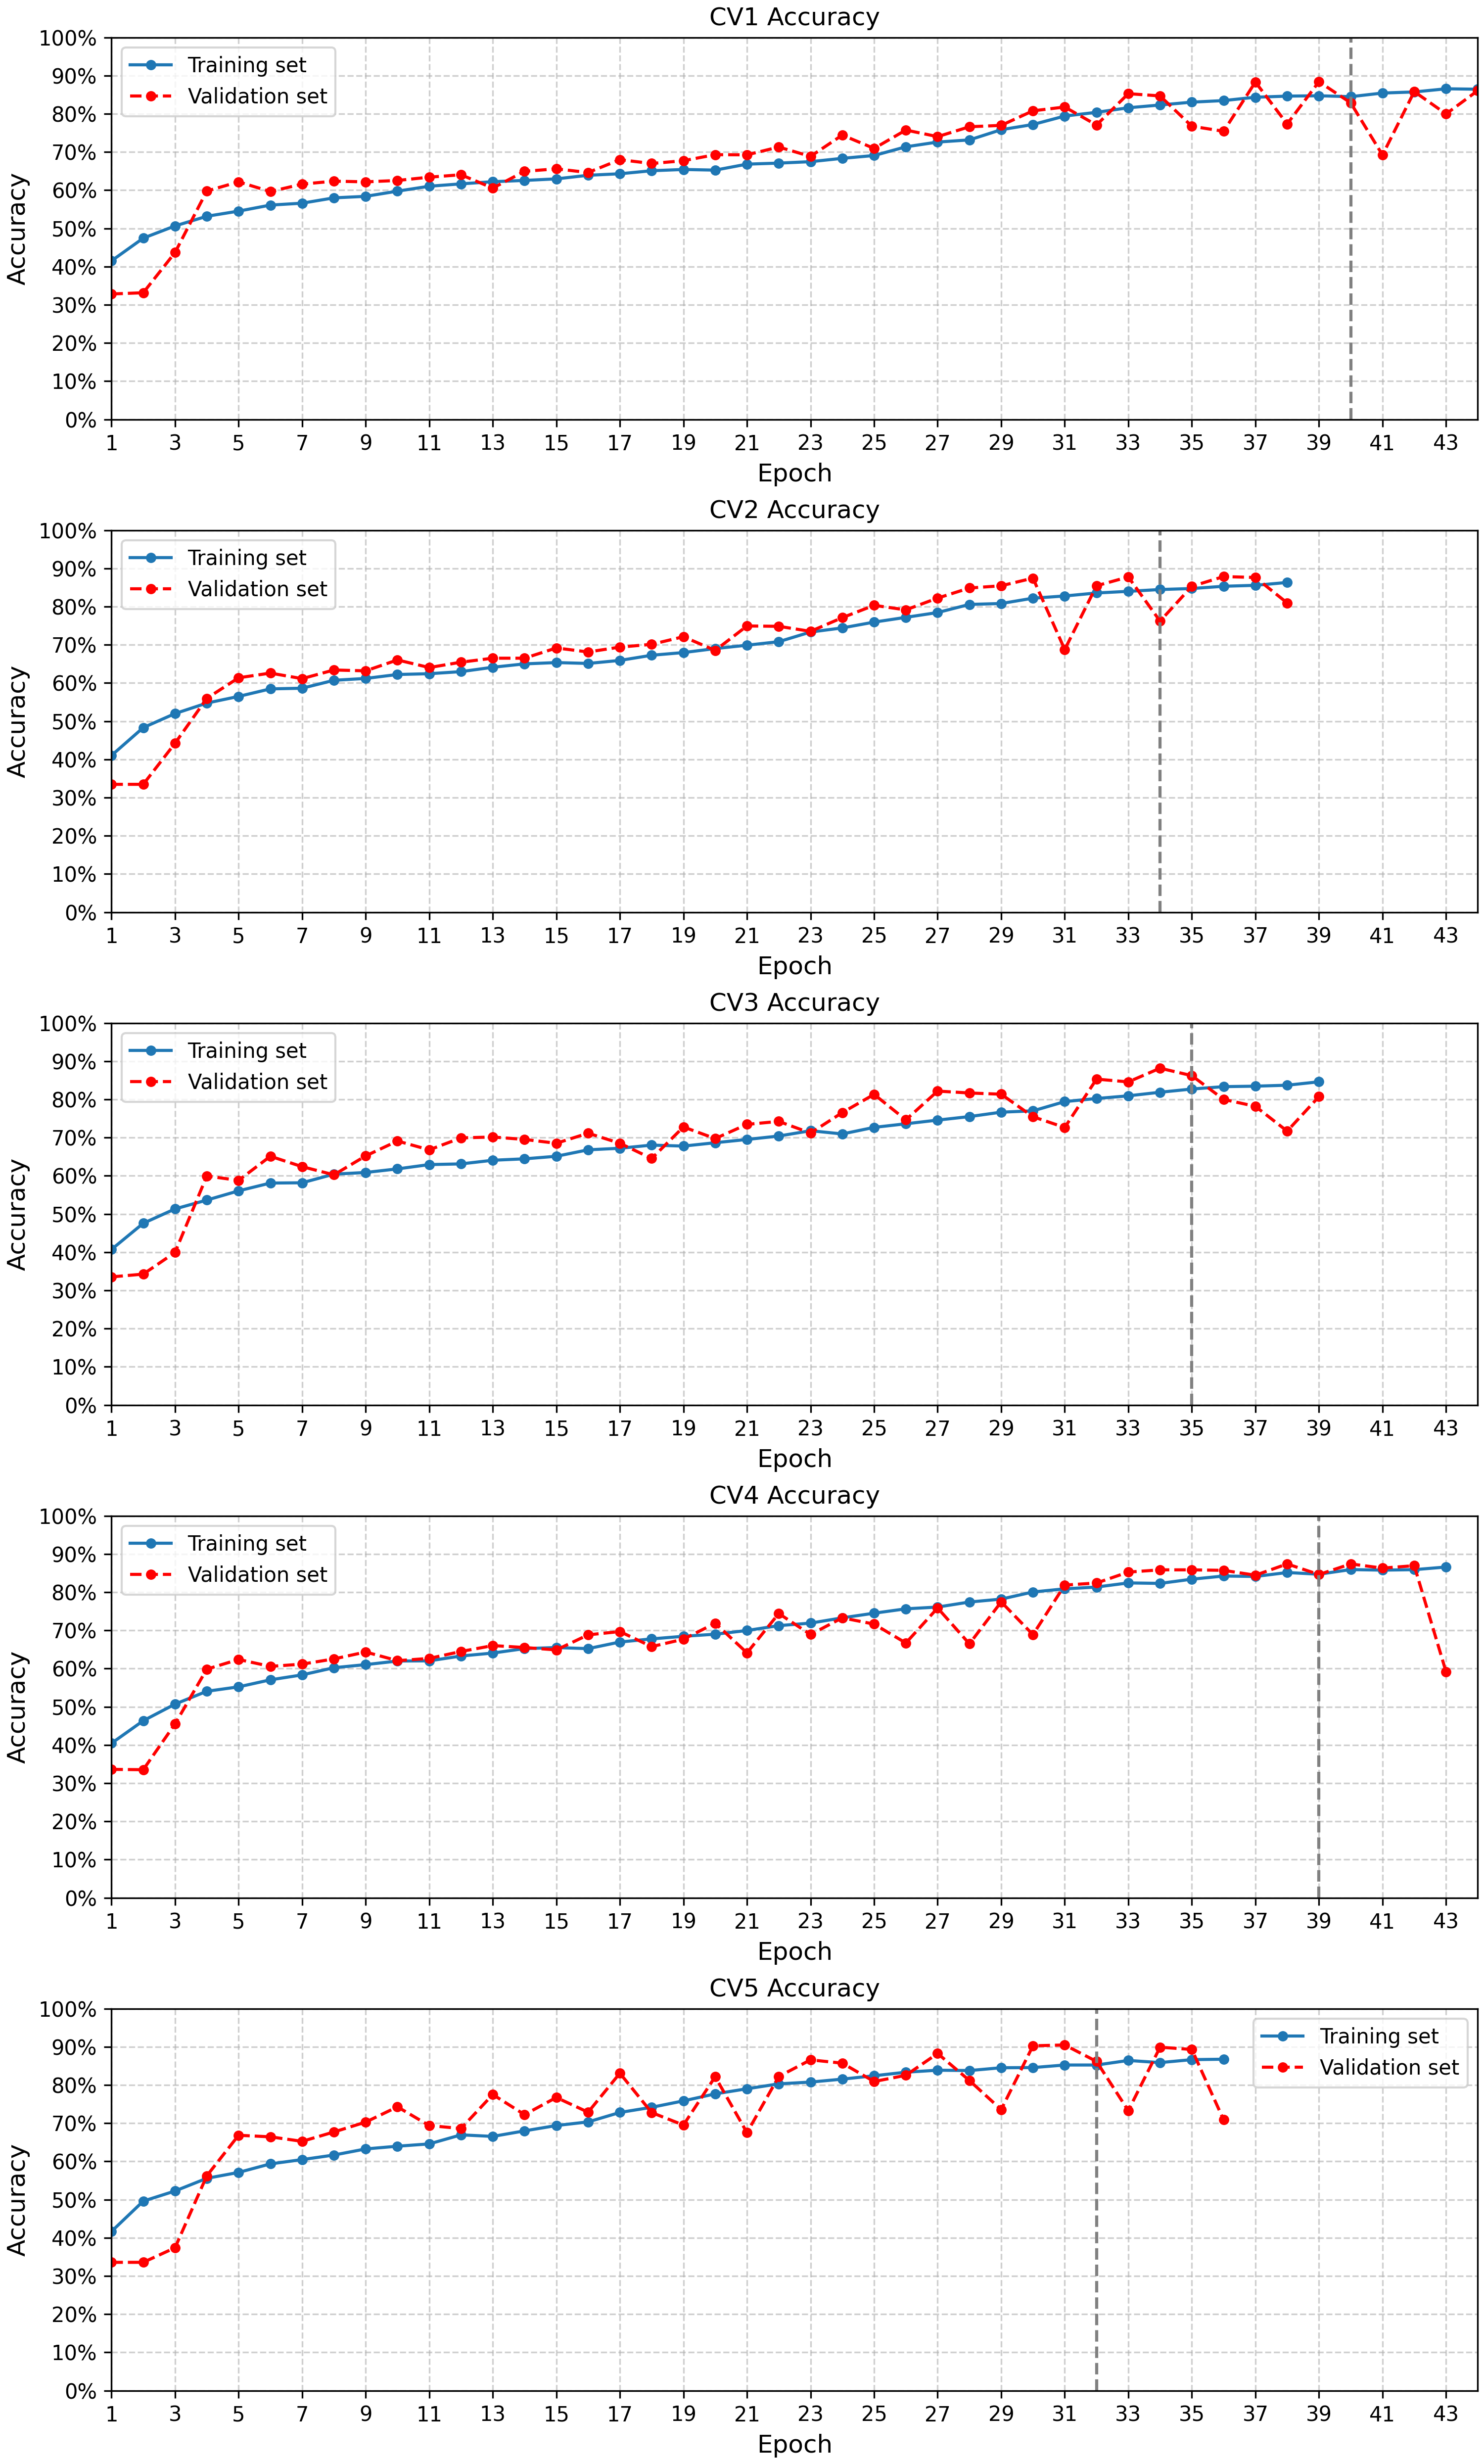
\includegraphics[width= 1.0\linewidth]{figures/bab4/akurasi_plotfix.png}
              \caption{Akurasi \textit{Training} Model}
              \label{Akurasi Training Model Terbaik}
          \end{figure}

          \begin{figure}[H]
              \centering
              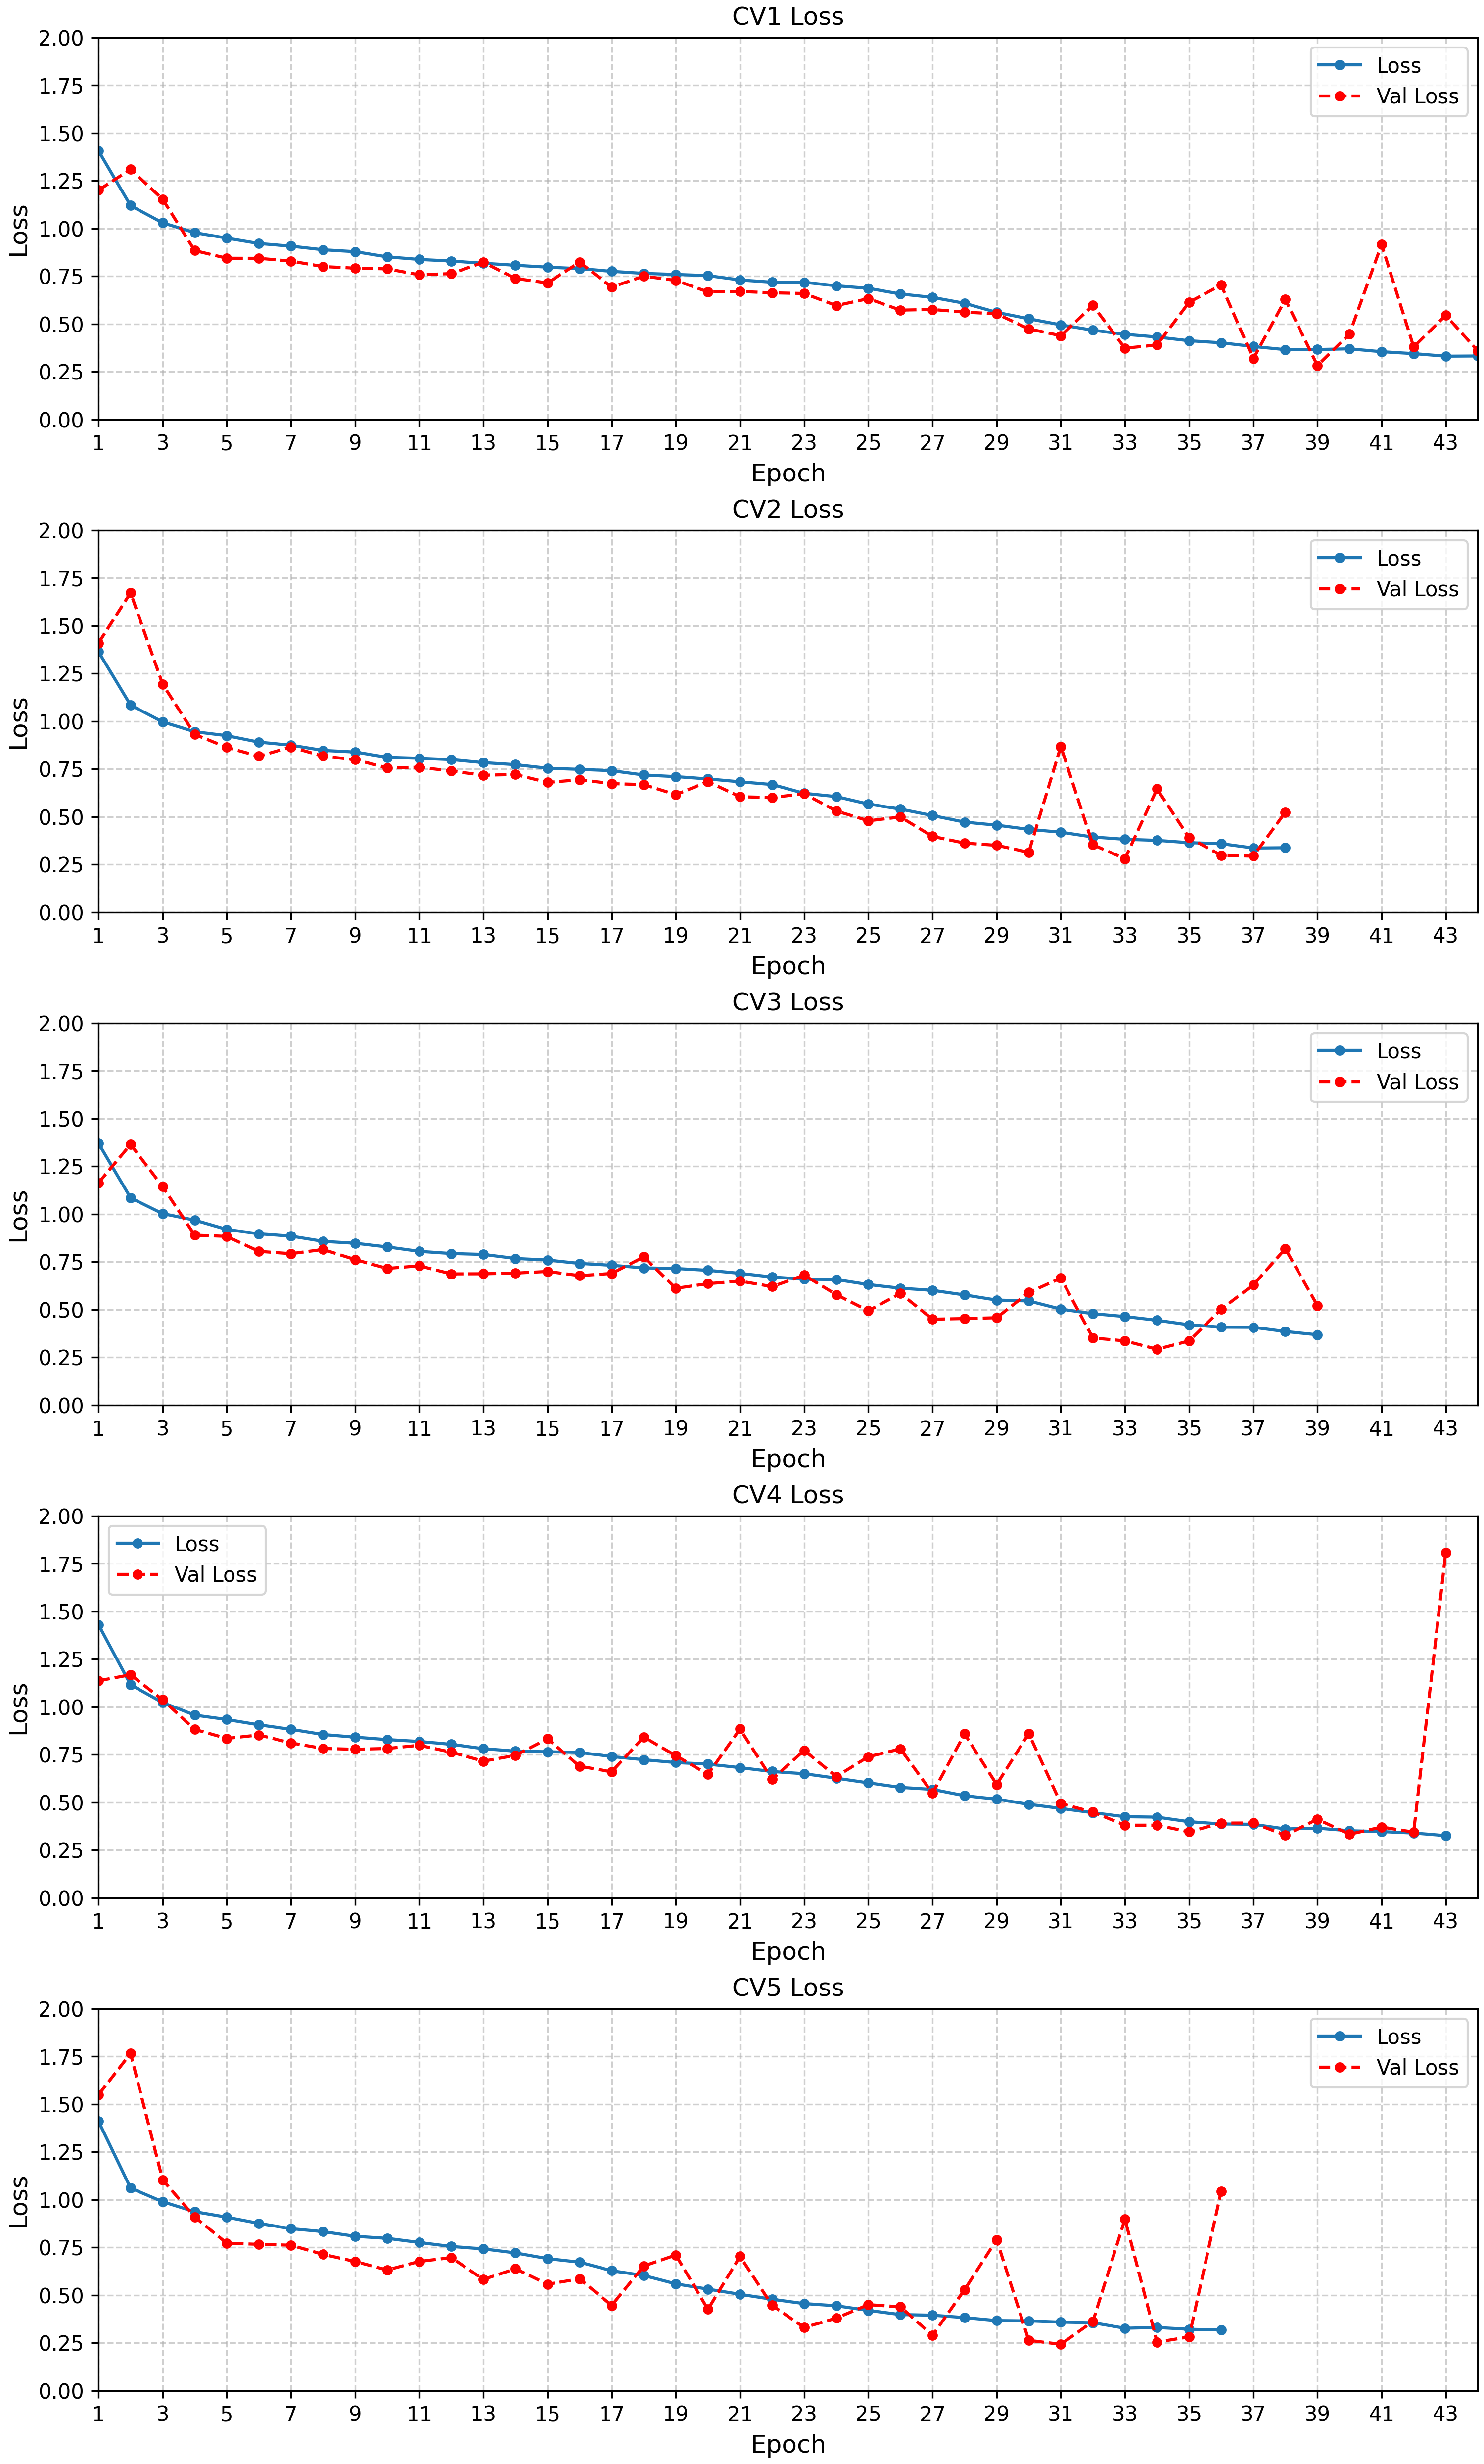
\includegraphics[width=1.0\linewidth]{figures/bab4/loss_plotfix.png}
              \caption{\textit{Loss Training} Model}
              \label{Loss Training Model Terbaik}
          \end{figure}

    Dapat dilihat akurasi dan \textit{loss} stabil di semua \textit{fold}, semakin tinggi nilai \textit{epoch} akurasi semakin meningkat dan akurasi di atas 90\%. Begitu juga dengan nilai \textit{loss} semakin tinggi \textit{epoch} semakin mengecil nilai \textit{loss} yang dihasilkan dan mendekati nilai nol.  Hal ini menunjukkan bahwa model mampu belajar dari data dan tidak hanya menghafal data pelatihan. Ini berarti model memiliki kinerja baik pada data baru yang tidak dilihat saat pelatihan.



  \subsection{Evaluasi Hasil}

        Pada tahap selanjutnya model di uji menggunakan data \textit{test} yang merupakan data baru yang tidak dilihat pada saat pelatihan. Hasil \textit{testing} model ditampilkan pada Gambar \ref{akurasi model terbaik} berikut.

          \begin{figure}[H]
              \centering
              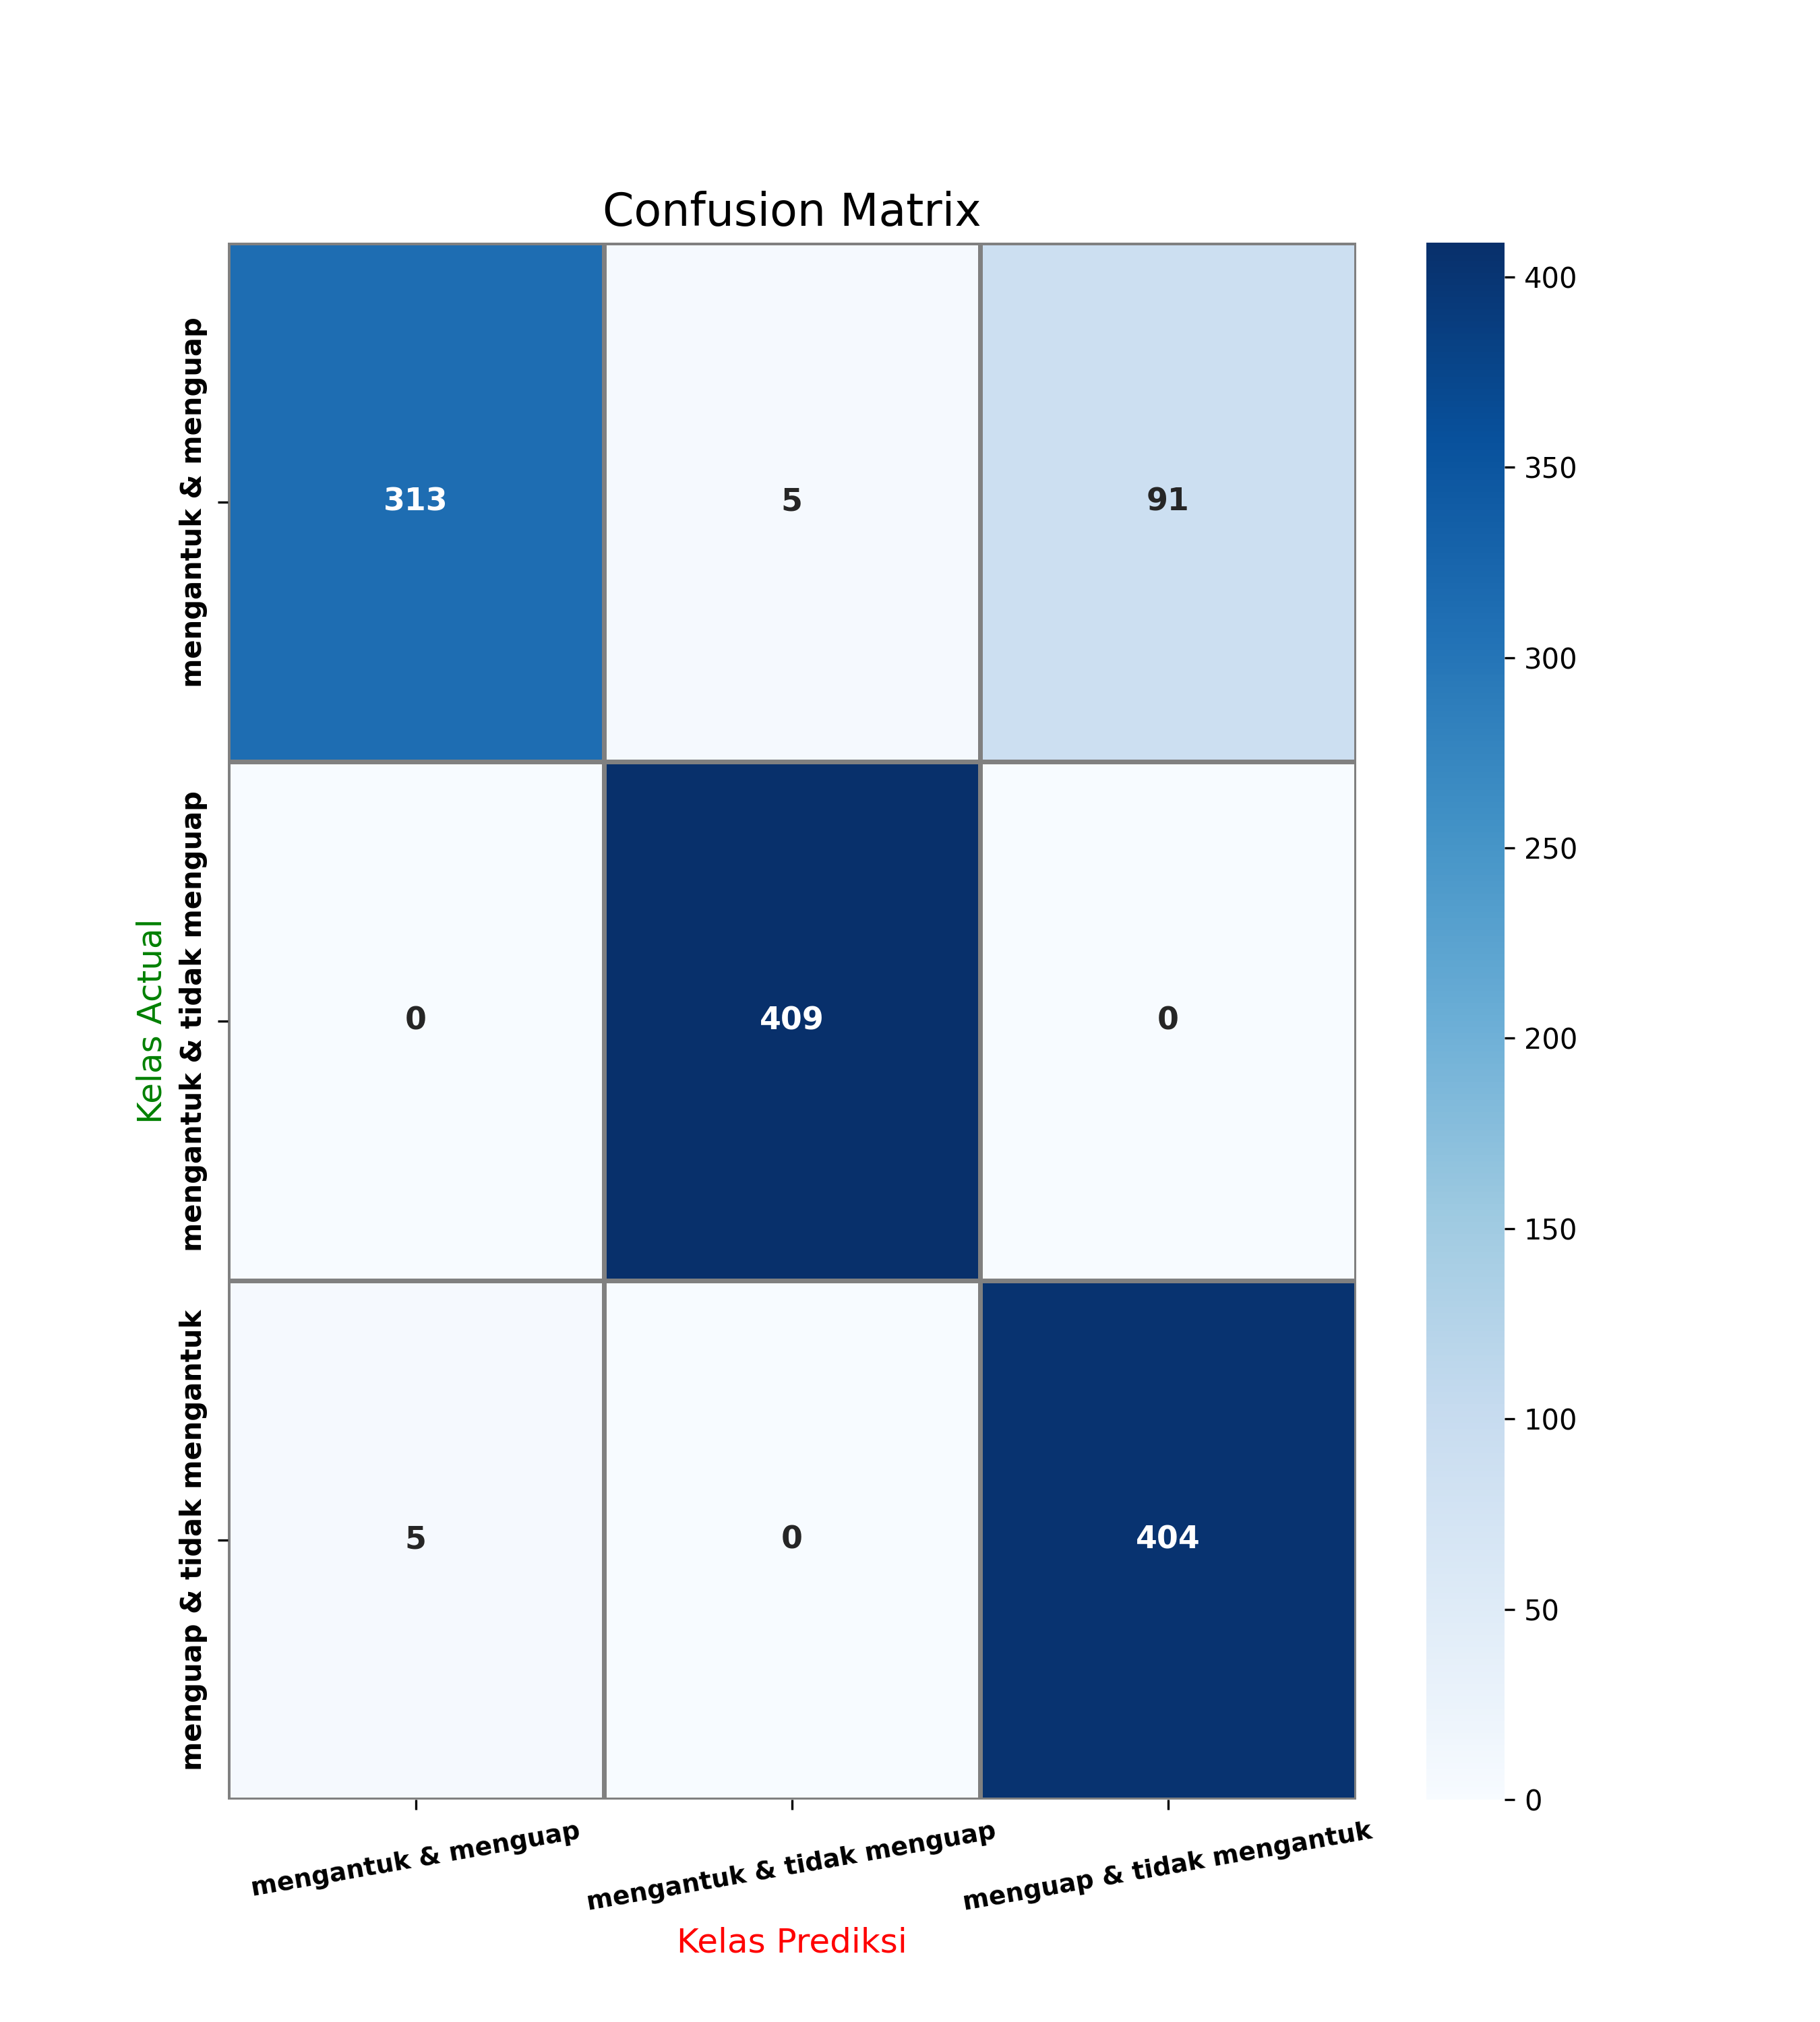
\includegraphics[width=0.75\linewidth]{figures/bab4/confusion matriks.png}
              \caption{Performa Matriks Model CNN}
              \label{akurasi model terbaik}
          \end{figure}

        Dapat dilihat dari hasil evaluasi menggunakan \textit{confusion matrix}. Nilai akurasi dan metriks yang dihasilkan tidak berbeda jauh dengan pengujian yang dilakukan sebelumnya. Hasil evaluasi ditampilkan pada Tabel \ref{Evaluasi Model} berikut.


        \begin{table}[H]
        \centering
        \caption{Evaluasi Model}
        \begin{tabular}{lccccc}
            \toprule
            \textbf{\textit{Kelas}} & \textbf{\textit{Recall}} & \textbf{\textit{Precision}} &\textbf{\textit{F1-Score}} & \textbf{\textit{Support }}\\
            
              & \textbf{(\%)} & \textbf{(\%)} & \textbf{(\%)} \\
            \midrule
            Mengantuk \& Menguap & 98.42 & 76.52 & 86.10 & 409 \\
            Mengantuk \& Tidak Menguap & 98.79 & 100.00 & 99.39 & 409 \\
            Menguap \& Tidak Mengantuk & 81.61 & 98.77 & 89.37 & 409 \\ \hline
            & & & & \\
            Accuracy & & & \textbf{91.76} & 1227 \\
            Average & 92.94 & 91.76 & 91.62 & 1227 \\
      
          
             \bottomrule
        \end{tabular}
        \label{Evaluasi Model}
    \end{table}

    Untuk hasil prediksi ditampilkan pada Gambar \ref{hasil prediksi} berikut.
         
          \begin{figure}[H]
              \centering
              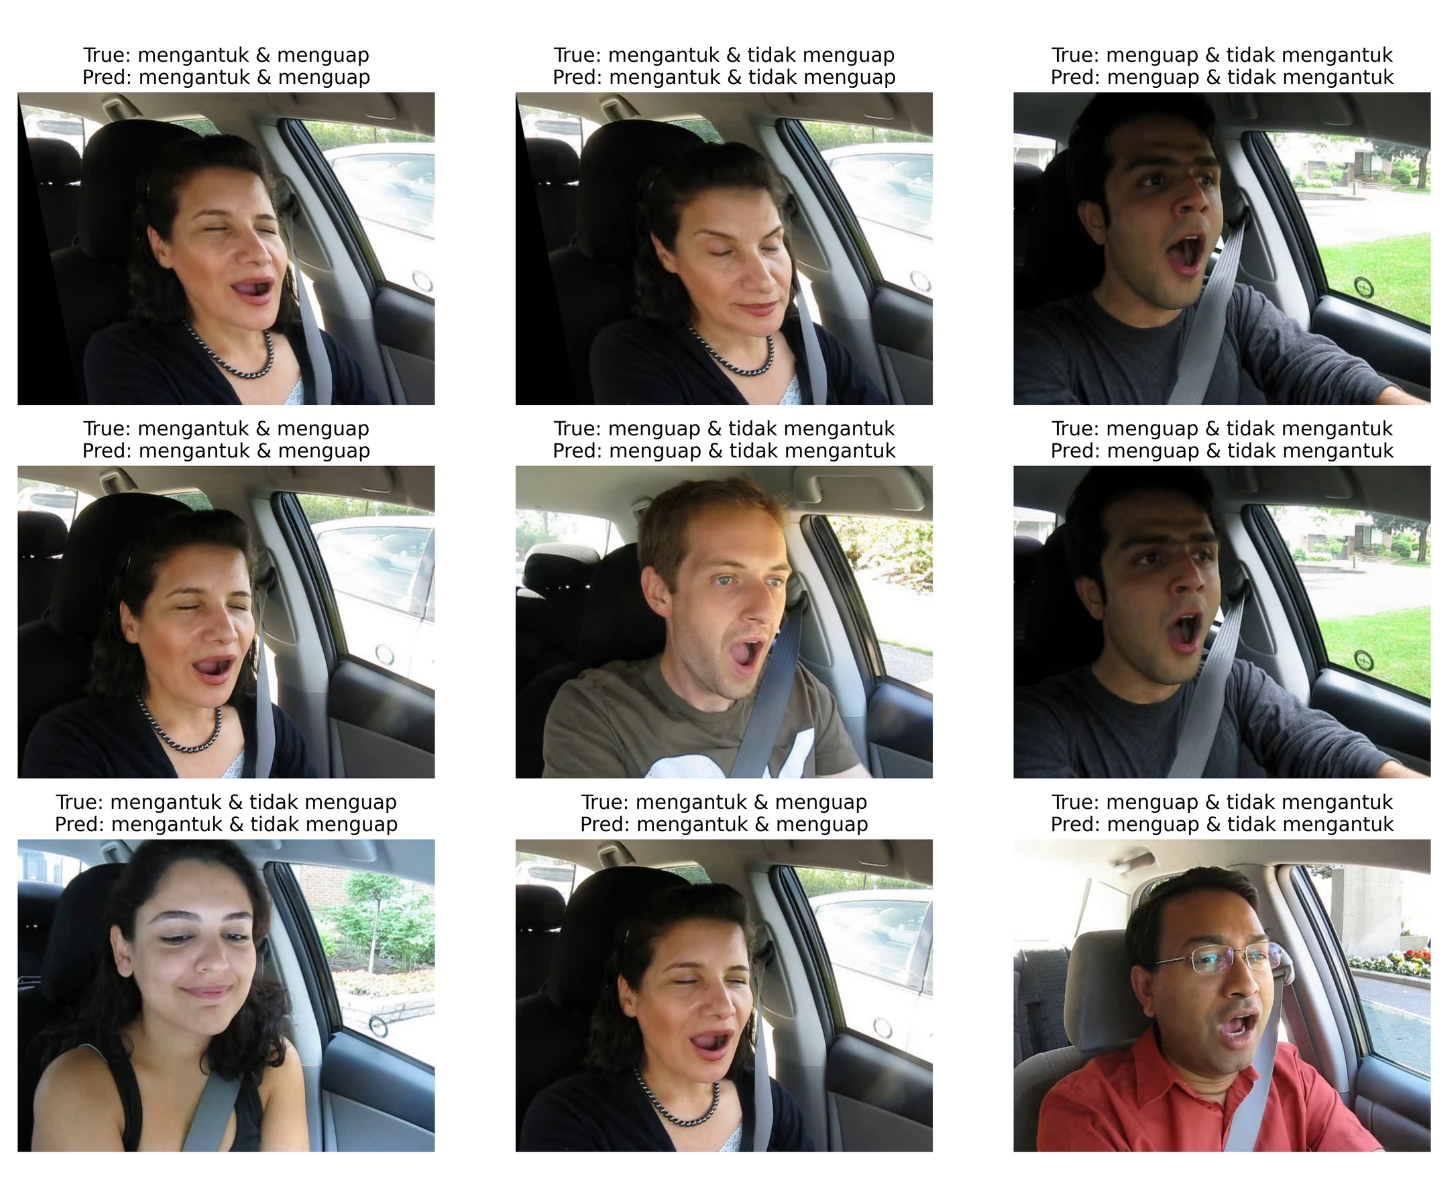
\includegraphics[width=1.0\linewidth]{figures/bab4/hasil_prediksi.png}
              \caption{Hasil prediksi}
              \label{hasil prediksi}
          \end{figure}

    
        
        
    Berdasarkan hasil percobaan yang telah dilakukan jika dibandingkan
     dengan penelitian sebelumnya yang dilakukan oleh Fiaz Majeed, dkk \cite{majeed2023detection}. Akurasi penelitian sebelumnya lebih tinggi dibandingkan penelitian ini, hal ini disebabkan adanya perbedaan segmentasi data, jumlah kelas dan metode yang dilakukan merupakan kombinasi antara CNN dan RNN. Ringkasan penelitian sebelumnya dapat dilihat pada Tabel \ref{Penelitian lama} berikut. 


    \begin{table}[H]
        \centering
        \caption{Penelitian Deteksi Kantuk Sebelumnya \cite{majeed2023detection}}
         \label{Penelitian lama}
        \begin{tabular}%{p{0.5cm}p{1.8cm}p{2.9cm}p{1.1cm}p{4.1cm}p{1cm}}
              {  >{\raggedright\arraybackslash}p{0.5cm} 
        >{\raggedright\arraybackslash}p{3 cm} 
        >{\raggedright\arraybackslash}p{2cm} 
        >{\raggedright\arraybackslash}p{5.0cm} 
        >{\raggedright\arraybackslash}p{1.0cm}}
    
            \hline
            \textbf{No}  & \textbf{Topik} &\textbf{ Metode} & \textbf{Hasil} & \textbf{Tahun} \\
            
            \hline
             1 
            &
            \textit{Detection of Drowsiness among Drivers Using Novel Deep Convolutional Neural Network Model}
            & 
            CNN \& RNN
            &
            
             Segmentasi data dilakukan dengan nilai MAR, dengan kelas yang diterapkan berupa \textit{binary class}. Eksperimen menunjukkan bahwa model mencapai akurasi rata-rata 96,69\% .
            &
            2023 \\   
            \\

             \hline

        \end{tabular}
    \end{table}


    Penelitian ini menghasilkan akurasi yang lebih rendah dibandingkan sebelumnya yaitu sebesar 91.76 \%. Hal ini terjadi karena pada penelitian ini menggunakan segmentasi data dengan nilai EAR dan MAR sedangkan sebelumnya hanya MAR. Penelitian ini juga menggunakan \textit{Multi-Class} sehingga jumlah model lebih sulit melakukan klasifikasi.

        \begin{table}[H]
        \centering
        \caption{Penelitian Deteksi Kantuk Baru}
         \label{Penelitian lama}
        \begin{tabular}%{p{0.5cm}p{1.8cm}p{2.9cm}p{1.1cm}p{4.1cm}p{1cm}}
              {  >{\raggedright\arraybackslash}p{0.5cm} 
        >{\raggedright\arraybackslash}p{3 cm} 
        >{\raggedright\arraybackslash}p{2cm} 
        >{\raggedright\arraybackslash}p{5.0cm} 
        >{\raggedright\arraybackslash}p{1.0cm}}
    
            \hline
            \textbf{No}  & \textbf{Topik} &\textbf{ Metode} & \textbf{Hasil} & \textbf{Tahun} \\
            
            \hline
             1
            & 
            Deteksi Kantuk Pengendara Mobil Menggunkan \textit{Convolutional Neural Networks} (CNN)

            & 
            CNN
            &
            Segmentasi data dilakukan dengan nilai EAR dan MAR, dengan kelas yang diterapkan berupa \textit{multi class} dengan hasil akurasi sebesar 91.76\%

            &
            2024 \\

             \hline

        \end{tabular}
    \end{table}

